%TC:group ocamlcode-in 0 0
%TC:group table 1 1
%TC:group tabular 1 1
\documentclass[12pt,notitlepage,a4paper]{report}

\usepackage{mydiss}
% \usepackage{euler}
% \includeonly{chapters/introduction}
% \includeonly{chapters/introduction,chapters/preparation,chapters/implementation,chapters/conclusion}
% \includeonly{chapters/introduction,chapters/preparation,chapters/implementation,chapters/evaluation}
% \excludeonly{chapters/evaluation,chapters/appendices/documentation}
%TC:ignore

\begin{document}
%%%%%%%%%%%%%%%%%%%%%%%%%%%%%%%%%%%%%%%%%%%%%%%%%%%%%%%%%%%%%%%%%%%%%%%%
% Title
\pagestyle{empty}

\hfill{\LARGE \bf Anik Roy}

\vspace*{\fill}
\begin{center}
	\huge
	\textbf{A probabilistic programming language in Ocaml}\\
	\vspace*{8mm}
	{\LARGE Computer Science Tripos - Part II} \\
	{\LARGE Christ's College} \\
	{\LARGE \today}
\end{center}
\vspace*{\fill}

\cleardoublepage

%%%%%%%%%%%%%%%%%%%%%%%%%%%%%%%%%%%%%%%%%%%%%%%%%%%%%%%%%%%%%%%%%%%%%%%%%%%%%%
% Proforma, table of contents and list of figures

\setcounter{page}{1}
\pagenumbering{roman}
\pagestyle{plain}


\chapter*{Declaration of Originality}

I, Anik Roy of Christ's College, being a candidate for Part II of the Computer Science Tripos, hereby declare that this dissertation and the work described in it are my own work, unaided except as may be specified below, and that the dissertation does not contain material that has already been used to any substantial extent for a comparable purpose.

I, Anik Roy of Christ's College, am content for my dissertation to be made available to the students and staff of the University. 

\bigskip
\noindent Signed: \raisebox{-1ex}{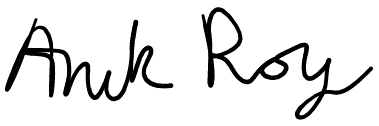
\includegraphics[trim=0 0cm 0 0,height=1.5\baselineskip]{figs/signature.png}}

\medskip
\leftline{Date:  \today}


\clearpage
\immediate\write18{texcount -inc -sum -1 diss.tex > wordcount.txt}
\immediate\write18{cloc  --yaml `git ls-files ..` | grep 'code: ' | tail -n 1 | sed  's/  code://g'}

{\large

\begin{tabular}{ll}
Candidate Number:               &  Anik Roy                       \\
College:            &  Christ's College                     \\
Project Title:      &  A Probabilistic Programming \\
&
 Language in Ocaml \\
Examination:        & Computer Science Tripos Part II        \\
Word Count:  
& \input{wordcount.txt}\footnotemark[1]\\
Final Line Count:         & \input{linecount.txt}\footnotemark[2] \\
Project Originator: & Dr R.~Mortier                    \\
Supervisor:         & Dr R.~Mortier                    \\ 
\end{tabular}
}
\footnotetext[1]{This word count was computed by \texttt{texcount -inc -sum -1 diss.tex}}
\stepcounter{footnote}


\footnotetext[2]{This line count was computed by \texttt{cloc (git ls-files)} and excludes blank lines and comments}
\stepcounter{footnote}

\section*{Original Aims of the Project}

\section*{Work Completed}

\section*{Special Difficulties}
None




\newpage

\cleardoublepage

\tableofcontents
\listoffigures
\listoflistings
\listoftables
\cleardoublepage

%%%%%%%%%%%%%%%%%%%%%%%%%%%%%%%%%%%%%%%%%%%%%%%%%%%%%%%%%%%%%%%%%%%%%%%
% main chapters

\setcounter{page}{1}
\pagenumbering{arabic}
\pagestyle{headings}

%TC:endignore
% !TeX root = ../diss.tex
\section{Motivation}

Creating statistical models and performing inference on these models is an important part of data science. A probabilistic programming languages (PPL) is a language used to create models, and allow inference to be performed on these models automatically. This allows the problem of efficient inference to be abstracted away from the specification of the model, and means inference code does not have to be hand-written for every model, making the task of designing models easier. The inference `engine' can also implement many different inference algorithms, which will each be more or less well-suited to different types of models. The core idea is that we have a prior belief over some parameters, ($p(x)$) and a generative model ($p(y|x)$) which specifies the likelihood of data given those parameters. What we are interested in is the posterior, the (inferred) distribution over the parameters given the data we observe ($p(y|x)$). In general, this kind of Bayesian inference is intractable, so we must use methods which approximate the posterior.

PPLs usually allow us to create these `generative models' as programs. Writing such a program requires us to be able to sample from distributions. However, since generative models are built up by sampling from probability distributions, PPLs need some way of modelling this non-determinism. Being able to condition programs on data is the other key part of PPLs, since we are interested in the posterior, which is conditional on the data. Without conditioning, we can run a program `forwards', which essentially means generating samples using the model we write. However, when we include a condition operator, we can infer the distribution of the input parameters based on the data we observe.

PPLs can either be standalone languages or be embedded into some other language. Embedding a PPL into a pre-existing language allows us to utilise the full power of the `host' language, and gives us access to operations in the host language without having to implement them separately. This makes it easier to combine models with each other as well as integrate them more easily into other programs written in the host language. Embedding a DSL into OCaml allows us to represent a wide range of models using OCaml's inbuilt functions and operators, and lets us leverage OCaml features such as an expressive type system or efficient native code generation.


\section{Related works}
There are many examples of PPLs, even as DSLs in OCaml. Some PPLs choose to limit the models that can be expressed in them in order to make inference more efficient, for example HANSEI in OCaml can only represent discrete distributions \cite{kiselyov2009embedded}. Others, such as STAN or infer.NET (F\#) can only operate on finite models (factor graphs), and do not allow unbounded recursion when defining models. Some, such as Church or Pyro, can express more general models, and are therefore known as `universal' \cite{} but often make the trade-off of less predictable or slower inference \cite{}.
% explain factor graphs here?

% mention what has been done - core and some extensions
% (here or abstract)


% TODO: mention "challenges", show non-trivial
% !TeX root = ../diss.tex

In this chapter, I will discuss the research done before starting the project, and some of the design decisions made based on this. In particular, common patterns in OCaml (and functional programming in general), influenced the final DSL, as well as the design of other similar probabilistic programming systems.

\section{Starting Point}

There do exist PPLs for OCaml, such as IBAL \cite{kiselyov2009embedded}, as well as PPLs for other languages, such as WebPPL - JavaScript\cite{mobus2018structure}, Church - LISP\cite{goodman2012church} or Infer.Net - F\#\cite{wang2011using} to name a few. My PPL can draw on some of the ideas introduced by these languages, particularly in implementing efficient inference engines. I will need to research the different approaches taken by these PPLs and decide what form of PPL to implement, especially in deciding the types of model I will want my PPL to be able to represent and the inference methods I implement.

I will be using an existing OCaml numerical computation library (Owl). This library does not contain methods for probabilistic programming in general, although it does contain modules which will help in the implementation of an inference engine such as efficient random number generation and lazy evaluation.

I have experience with the core SML language, which will aid in learning basic OCaml due to similarities in the languages, however I will still have to learn the modules system. 1B Foundations of Data Science also gives me a basic understanding of Bayesian inference. I do not have experience with domain specific languages in OCaml, although the 1B compilers course did implement a compiler and interpreter in OCaml.

\section{Requirements}

Before starting to write any code, I made sure to set out the features I aimed to implement for my DSL. The main goal was to produce a usable language, which was defined by the following criteria:

% TODO: which tense to use here - past, say "this met the success criteria as follows"
\begin{itemize}
	\item \textbf{Language Features}: Since I have written an embedded DSL, a user of my PPL should be able to take advantage of all standard OCaml features in the deterministic parts of their models. I need to make sure that this is the case, and features such as recursive functions will work.
	\item \textbf{Available distributions}: I aimed to make sure my PPL has at minimum the Bernoulli and normal distributions available as basic building blocks to build more complex probabilistic programs.
	\item \textbf{Correctness} of inference: I used the PPL developed on example problems to ensure correct results are produced. These results were compared to results produced in other PPLs as well as comparisons to analytic solutions for simple problems.
	\item \textbf{Available Inference Algorithms}: I aimed to include at least one available inference algorithm. However, since different problems are more or less well suited to different general-purpose inference procedures, I wrote implementations for five separate algorithms.
	\item \textbf{Performance}: This is a quantitative measure, comparing programs written in my PPL to equivalent programs in other PPLs. I used the profiling tools spacetime and GProf to profile my OCaml code. Performing inference should be possible within a reasonable amount of time, even though the project does not have a significant focus on performance. I also benchmarked the performance with regards to scalability, i.e. made sure the performance is still reasonable as models are conditioned on more data.
\end{itemize}

\section{Professional Practice}

I adopted several best practices in order to ensure the project was successful. This includes performing regular testing, splitting code into separate modules designing signatures first, and ensuring my code follows a consistent style guide (Jane Street style\footnote{\url{https://opensource.janestreet.com/standards/}})

\subsection{Testing}

Testing systems which are linked to randomness can be quite tricky, as it is difficult to test behaviour that is expected to change from one execution to the next. One approach is to set a fixed random seed and make sure the same sequence of results are produced. The aim of a unit test, however, is to make sure that a desired property does not change from one version of the code to the next. Even with a fixed random seed, a change in code may cause new outputs even though the fundamental statistical property desired hasn't changed. Another approach is to perform some statistical test such as kolmogorov-smirnov \cite{massey1951kolmogorov}, to ensure distributions produced by my library are equal to what is expected. A problem with tests of this kind is that they are expected to fail sometimes, meaning unit tests will provide limited utility due to their inherent flakiness with random programs. In fact, since we expect these tests to fail a certain percentage of the time, if they do not sometimes fail there is a problem with our program.

As such, most of the unit tests I wrote are fairly simple and only catch very basic bugs. Unit tests were possible to write for the exact inference procedure when working with discrete distributions, since we always expect the same output distribution. However, all the other inference algorithms are approximate, so tests suffer from the problems described above. I was still able to carry out a full evaluation, performing hypothesis tests such as the kolmogorov-smirnov or chi-squared tests.

However, there are several auxiliary functions that can be tested effectively using conventional methods, so I was able to test them as normal. I also used the \texttt{Quickcheck} library to perform tests using randomised data, which allows me to ensure certain invariants are preserved by functions.


% talk about using very basic unit tests
% unit testing ppl is 
% include maths about hypothesis tests here - HAVE TO FAIL SOMETIMES otherwise the program is wrong
% include unit tests for exact inference
% go though how to solve this in implementations
% find some sources for how other people solve this, reference that here.

\subsection{Continuous Integration}
Since I will be developing a library, it is important to make sure that any unit tests are run regularly to ensure there are no regressions - no new code affects old behaviour. It is also important to make sure the library will function on different platforms, and that documentation is built (and possibly uploaded) automatically. To achieve this, I will be using GitHub's continuous integration service, `actions' to make sure the code on the master branch always works. The CI can also be used to ensure the library works with older versions of OCaml, and is backwards-compatible.

\subsection{Licenses}

The major libraries I use, Owl and Jane Street Core, are both licensed under the MIT license.
% what else do i write here - the pink book says to talk about licenses

\section{Tools and Technologies}
The main tools I used are listed here:
\begin{itemize}
	\item Ocaml 4.08 - The language I wrote the main PPL library in
	\item Dune - Build system for OCaml
	\item Opam - OCaml package manager
	\item Alcotest - Unit testing framework
	\item Quickcheck - Random testing library
	\item Spacetime - Memory profiler for OCaml
	\item Landmarks - Profiler for OCaml
	\item Owl - Scientific computing library in OCaml
	\item VSCode (with ocaml extensions) - IDE for OCaml development
	\item Git with GitHub - version control
\end{itemize}

Using OCaml 4.08 allows me to use new features of OCaml, in particular the ability to define custom let operators as syntax sugar for monads. The dune build system also allows me to more easily manage building and testing my code, as well as automatically creating documentation from comments and function signatures in my code. The profilers I used allowed me to work out the causes of performance issues and remedy them. 

\section{OCaml}
I have chosen to use the OCaml language to implement my PPL. There are many features of OCaml which make it suitable for writing a DSL. Using OCaml, I can make sure that expressions in the DSL are well-typed, so that programs don't fail to run. OCaml's algebraic datatypes also make it easy to represent probabilistic programs as trees, and pattern matching makes it easy to 'interpret' and transform these trees. The module system also makes sure that certain types are hidden from the user, which can ensure only valid structures are created by the user.

\subsection{GADTs}
The main data structure I use to represent distributions is GADT - a generalised algebraic data type. GADTs are similar to ADTs (sum types), in that they have a set of constructors, but the main difference is that these constructors can have their output types annotated. The fact that the return types of constructors can vary is what makes GADTs more general than normal ADTs, whose return types are all the same. In OCaml, the syntax for this is \texttt{type \_ t = Constructor : type' -> type' t | ...}. Since we can now know which constructors produce which types of t (e.g. an \texttt{int t} or a \texttt{float t}, etc.), functions can be defined to only accept certain constructors, and we can make sure the whole structure is well typed.

\subsection{Monads}
% how in-depth should my explanation of a monad be?
Monads are a design pattern commonly used in functional programming languages.

The key data structure I use to model probability distributions is a monad. A data type is a monad if it defines two operations, \texttt{return} and \texttt{bind}, and can be thought of as datatypes which `wrap' values. The return function takes a value and returns a monad wrapping that value. The bind function takes a monad and a function, and applies the function to the value wrapped inside the monad, and rewraps this value. The type must also satisfy a set of laws, which I omit here\cite{wadler1990comprehending}. Monads can be used to structure programs in a general way, and allow side effects to be described in a pure way.

\subsubsection{Probability Monad}
It has been shown that probability distributions form a monad, \cite{giry1982categorical} \cite{jones1989probabilistic}, and that they can be used to create composed distributions \cite{ramsey2002stochastic}. In this case, \texttt{return x} represents a distribution with only one value, x (technically a Dirac distribution), and \texttt{bind d f} is the main operator for composing distributions. Binding distributions together represents taking the output of one distribution and using it in the body of the function.

\subsubsection{Custom let operators}
Ocaml 4.08 allows me to define definitions for custom let operators. This is used to provide syntactic sugar for working with monads, and is similar to do-notation in Haskell. The reference documentation \footnote{\url{http://caml.inria.fr/pub/distrib/ocaml-4.08/ocaml-4.08-refman.html}} outlines this, and a monad should provide a module which implements the (let*) and (and*) operators. The (let*) operator is the standard bind function - here it takes the identifier bound to as the first argument to the function in bind. The (and*) operator is the product operation, it takes two monads and returns the monad pair - it has signature \texttt{'a m -> 'b m -> ('a*'b) m}, where m is the monad type. An example, using the Option monad is given below to show the transformation that takes place. This syntax allows the user to not have to use the bind (or the alias >>=) explicitly, and offers a more intuitive syntax.

\ocamlcode{code_snippets/let_syntax.ml}

\subsection{Modules}
The module system is a key feature of the OCaml language. Every function in OCaml is in a module, by default the name of the file it resides in. Modules can also have signatures, which define what code is visible to a user, and constrain the module. This allows modules to hide types and implementations to provide a clean API. Modules are often used to wrap a particular type, for example a list or map. This means that to create or manipulate that type, the user must go through the modules API, ensuring only permitted operations are carried out. This is a feature I've used in designing distribution types. Modules can also be dynamically created from other modules, using functors, which are functions from modules to modules. This technique is used extensively in the Core library, and it allows modules to be customised and extended.

In OCaml, the module language (functors, modules, signatures, etc.) and the core language (functions, values, types, etc.) are considered separate, and values can't contain modules. First class modules provide a way around this constraint, and allows modules to be used in much the same way as ordinary values. This allows us to simplify the creation of modules from the users point of view, and means a library can define functions to create modules which can then be used by other functions.

\section{Owl}

Owl is a scientific computing library written for OCaml \cite{owl}. Importantly for my PPL, it contains functions for working with multi-dimensional arrays, as well as a wide variety of statistical functions. In particular, it contains functionality relating to many common distributions, e.g. normal, beta, binomial, etc. Since my language will allow the user to combine these basic distributions into larger models, I will need to use these functions to allow sampling from and the ability to perform inference on these models. In particular, it is important to be able to find the probability density function (pdf) and cumulative density function (cdf) of these distributions as well as sample from them. Another important feature of owl is it's plotting functionality which enabled me to write functions which let me visualise output distributions, as well as visualising performance statistics, all directly from OCaml.

\section{Approaches to probabilistic programming}
Existing PPLs take several different forms, both as standalone and embedded languages. The main trade-off that is made in the design of PPLs is the number of models that can be expressed in the language compared to how efficient inference is. One approach is graph-based, where a \textit{factor graph} is generated from the program, over which efficient inference can take place. This approach can be seen in languages such as infer.NET or JAGS, and has the benefit of very fast inference, particularly since efficient computation graph frameworks can be leveraged - an example is Edward \cite{edward}, which uses TensorFlow as a backend. However, these languages usually cannot represent infinite models or unbounded recursion. Another approach, taken by the likes of WebPPL or Anglican, is trace-based. This approach considers execution traces, with a `trace' being one run of a program, with all the intermediate variables taking a particular value. Inference algorithms can reason about these traces in order to produce a posterior distribution, as will be seen in the next section. A trace-based approach often leads to clearer programs, since we are not working with a computation graph. It also leads to more models being able to be expressed, since we are not limited by the constraints of a graph. However inference is often slower, particularly when dealing with data in high dimensions, since the algorithms need to be more general purpose, and often converge slower.

\section{Bayesian Inference}
Inference is the key motivating feature of probabilistic programming, and is a way to infer a distribution over the parameters based on the data we observe. The main feature of Bayesian inference is that we assign every model some prior belief. Often this prior is chosen based on our knowledge of the problem, but the prior can also be uninformative. The goal of Bayesian inference is to calculate the posterior distribution, which can be represented by Bayes' formula,


$$P(A\mid B)={\frac {P(B\mid A)P(A)}{P(B)}}$$

with $P(A)$ being the prior, and $P(B\mid A)$ being the likelihood model we define. In the PPL setting, the prior is the generative model we define, with condition statements defining the likelihood. Running inference on the program then produces a sampler for the posterior.

This formula hold for the continuous case too, using probability density functions ($f_X$),

$$ f_{X\mid Y=y}(x)={\frac {f_{Y\mid X=x}(y)f_{X}(x)}{f_{Y}(y)}} $$

Unfortunately, exact Bayesian inference is usually computationally infeasible, especially when the number of random variables we consider is large. For example, consider a set of discrete random variables ${X_i}$, with p the joint probability distribution of all $X_i$. The marginal distribution of any individual $X_i$ is:

% How does this relate to the inference problem?
$$P(X_i=x) = \sum_{j=0}^{50} $$

If we have 50 variables which can take one of two values, then we have to sum over $2^{50}$ values. There do exist some algorithms which operate on Bayesian networks (DAGs which represent random variables and their interdependence), and reduce the number of calculations needed. These include methods such as \textit{Variable Elimination} or \textit{Message Passing} \cite{belief-prop} \cite{}.

Alternatively, in the continuous case the formula is

$$P(\theta\mid x)=\frac{P(x\mid\theta)P(\theta)}{P(x)}$$
with 
$$P(x)=\int_{\Theta}P(x,\theta)~d\theta $$

The normalizing constant here is an integral that often does not have an analytic solution, and so must be approximated. Another issue is that directly sampling from a distribution requires that we also invert this formula.

\section{Inference Algorithms}
% https://ermongroup.github.io/cs228-notes/inference/sampling/
% https://people.eecs.berkeley.edu/~jordan/courses/260-spring10/lectures/lecture17.pdf

% https://www.cs.ubc.ca/~fwood/teaching/OXWASP_CDT/probabilistic_programming.pdf
% http://www.robots.ox.ac.uk/~fwood/anglican/assets/pdf/Wood-AISTATS-2014.pdf
Inference algorithms are ways to systematically generate samples from posterior distributions given a likelihood function and a prior distribution. In probabilistic programming, a model consists of latent variables and observed variables, and a single execution of a model (a program) can be thought of as an assignment to each of these variables, known as an \textit{execution trace}. This can be defined mathematically as below, by Bayes' rule:
% 
$$p(x_{1:N}|y_{1:N})\propto \tilde{p}(y_{1:N},x_{1:N})$$ 
% 
Note that the trace may have a different number of variables each time a model is run, due to the fact that we allow general models which allow for unbounded recursion. 

Here, $p$ is the posterior distribution of a particular trace $x$, given the observed variables $y$. This is proportional to the joint distribution of all the variables ($\hat{p}$). The aim is then to find the posterior over the latent variables we are interested in (by marginalising the other variables). We can specify which variables we care about within the program, either as part of the model, or outside it in a query to the model.

\subsection{Exact Inference}

Exact Inference is the simplest method of calculating the posterior, but is usually computationally intractable. It involves calculating Bayes formula exactly, of which calculating the normalising constant is usually the problem. To sample directly, we would also need to find the inverse cumulative distribution to be able to use the inversion sampling method.

For discrete posterior distributions it can be thought of as calculating the probability of every possible value of the variable of interest. Since a random variable will be dependent on several others, this involves finding every possible combination of these variables and their outcomes.

\subsection{Rejection Sampling}

Since exact inference is too difficult in practice, we usually have to resort to \textit{Monte Carlo} \cite{monte-carlo} methods.

One such method, rejection sampling, is a very simple inference method which uses another distribution which \textit{can} be sampled from. We take samples from this distribution, and either accept or reject them based on whether

\subsection{Importance Sampling}

Importance sampling is another simple method, improving on rejection sampling, that can be used to sample from a target distribution using another distribution, known as the proposal distribution. We then calculate the ratio of the likelihoods between the two distributions to weight samples from the proposal. From doing this repeatedly with multiple samples from the proposal, we can build a posterior represented by a set of weighted samples.

% put proofs of inference methods here/implementation/appendix?
% Add equations

\subsection{Monte Carlo Markov Chains (MCMC)}

MCMC methods involve constructing a Markov chain with a stationary distribution equal to the posterior distribution. A Markov chain is a statistical model consisting of a sequence of events, where the probability of any event depends only on the previous event. The stationary distribution is the distribution over successive states that the chain converges to.

There exists several algorithms for finding this Markov chain, for example metropolis-hastings. This algorithm requires that we have a function, $f(x)$, which is proportional to the density of the distribution. The function is easy to compute for the posterior, since it is simply the prior multiplied by the posterior - the normalising constant can be ignored since we only need a proportional function.

MCMC algorithms have the same basic structure - to first `run' the chain for a burn-in period, taking samples and discarding them. Then, running the chain and collecting the states visited as samples. This set of samples is then a set of samples from the posterior, since the posterior should be equal to the stationary distribution. An important trade-off is made in the length of the burn-in period - too long and time is wasted discarding states, but too short and the chain will not converge to the correct distribution.

\subsection{Sequential Monte Carlo (SMC)}

SMC methods are algorithms which are based on using large numbers of weighted samples (`particles') to represent a posterior distribution. SMC methods are also known as particle filters. A particle is a value paired with an unnormalised weight which represents the likelihood of that value in the distribution. These particles are updated when data is observed and re-sampled from in order to converge the set of particles to the posterior.

The simplest SMC algorithm is the bootstrap filter\cite{particlefilter}, which simply resamples once on encountering new data, updating the weights of the particles based on how likely this data is deemed to be. However, many variations exist - the resampling method, updating the weights and the initial particles can all be varied. The main feature of SMC is that they sequentially create sets of particles which converge to the desired distribution.

SMC methods can also be combined with MCMC methods to create new algorithms. These algorithms are known as particle Monte Carlo Markov chain (PMCMC) algorithms, and were first introduced for probabilistic programming in the Anglican language \cite{anglican-smc}.
% !TeX root = ../diss.tex
\chapter{Implementation}
In this chapter I describe how the DSL is implemented. Documentation for all publicly exposed functions can be found in appendix \ref{app:docs}.

\section{Repository Overview}

\begin{wrapfigure}[25]{R}{0.4\textwidth}
	\dirtree{%
		.1 ppl.
		.2 \_build.
		.2 \_coverage.
		.2 bin.
		.3 \dots.
		.2 doc.
		.2 lib.
		.3 inference.
		.4 \dots.
		.3 dist.ml.
		.3 empirical.ml.
		.3 helpers.ml.
		.3 inference.ml.
		.3 monad.ml.
		.3 plot.ml.
		.3 ppl.ml.
		.3 primitive.ml.
		.2 test.
		.3 unit\_tests.
		.4 \dots.
		.3 test\_models.ml.
		.3 hypothesis\_tests.ml.
		.2 dune-project.
		.2 ppl.opam.
	}
	\caption{Directory structure}
	\label{fig:dirs}
\end{wrapfigure}

% TODO: include a file tree?
The majority of my code is in the \texttt{ppl} directory, which contains the core library, unit tests, statistical testing code and some example programs written using the library. A separate evaluation folder contains code to compare my ppl to other languages.

I have implemented my ppl as a library residing in the \texttt{lib} subdirectory, contained within the module \texttt{Ppl}. Opening this module in a script allows a user to use my library. Ppl includes several submodules, most importantly the \texttt{Dist} and \texttt{Inference} modules, which contains the code for representing, creating and combining distributions, and performing inference, respectively. These functions can be found in separate files in the inference folder, and are all exported in the inference module. The other modules exported in Ppl are plot, prim\_dist, and samples.

\texttt{Prim\_dist} contains code for using primitive distributions - as well as types which a user can provide to define their own distributions. It also defines functions which can be used by the user to create new primitive distributions.

The \texttt{Plot} module contains helper functions which wrap around Owl\_plplot, allowing users to easily create visualisations from distributions defined in my ppl. This includes histograms 

The \texttt{bin} directory contains several example programs to show how the ppl can be used to express many different models. 

The \texttt{test} directory contains basic unit tests as well as hypothesis tests to check the correctness of inference.

The \texttt{evaluation} directory contains code to compare my ppl to both hand-written inference procedures, as well as equivalent programs in other PPLs. There are several directories, which each correspond to a particular problem/model.

All code is written in OCaml 4.08, with the main dependencies being Jane Street's \texttt{Core} and \texttt{Owl} \cite{owl}.	
	
\section{Language Design}
I chose to implement my language as a domain specific language (DSL) shallowly embedded into the main OCaml language. This allows models built in the ppl to be easily composed with other standard OCaml programs.
	
Using a shallow embedding means we can use all of the features of OCaml as normal, including branching (if/then/else), loops, references, let bindings, (higher-order) functions, and importantly, recursion. This can allow us to define models that do not terminate and are therefore invalid. However, we can write functions which are \textit{stochastic recursive} \cite{siegmund}, that is, functions which have a probability of termination that tends to 1 as the number of successive calls tends to infinity. This leads to functions which terminate their recursion non-deterministically. Any model which does not satisfy this will be considered an invalid model - unfortunately as it is not possible to determine whether or not a program will halt, this property cannot be enforced. 
	
I use a set of primitive distributions which can be combined (using arbitrarily complex deterministic OCaml code) to produce new more complex distribution. For example, one can take the sum of two discrete uniform distributions to simulate the addition of two dice rolls. 
	
PPLs in general are similar to normal programming languages, but need to support two extra operations - \texttt{sample} and \texttt{condition} \cite{gordon2014probabilistic}. The sample operator allows models to be built up. The condition operator has a few variants, which are covered in section \ref{sec:condition}.
	
\section{Representing Distributions}
In order to define my DSL, I needed data structures to represent probabilistic models as well as distributions that are used as both input and output. Input distributions are the primitive distributions that are used to build models and constrain observations. We have more information about these distributions, such as how to sample from them exactly and exact pdf functions, and this information is used in inference. The output of inference is usually a distribution which can be sampled from to obtain the posterior, but we generally want to also collate statistics about the posterior distribution. Since we only have an approximate sampler, we can output empirical distributions from which many statistics, e.g. mean, variance, cdf etc., can be approximated.
	
\subsection{Probability Monad}
	
As mentioned before, monads are a natural way to represent probability distributions. They allow the output from one distribution (essentially a sample), to be used as if it was of the type that the distribution is defined over. Essentially, the \texttt{bind} operation allows us to 'unwrap' the 'a dist type to allow us to manipulate a value of type 'a. We must then use \texttt{return} to `wrap' the value back into a value of type 'a dist. The type signature of bind is \texttt{'a m -> ('a -> 'b m) -> 'b m}, and return is \texttt{'a -> 'a m}, with m being the monad type.
	
Using monads also allows us to define several helper functions which can be used when working with distributions. For example, we can `lift' operators to the \texttt{dist} type, for example allowing us to define adding two distributions over integers or floats using liftM or liftM2. We can also fold lists of distributions using a similar technique.
	
Using monads also allows the use of the extended let operators introduced in OCaml 4.08. These allow the definition of custom let operators, which mimic do-notation in Haskell. This means that sampling from a distribution (within a model) can be done using the \texttt{let*} operator, and the variable that is bound to can be used as if it were a normal value. The one caveat is that the user must remember to \texttt{return} at the end of the model with whatever variable(s) they want to find the posterior over. The \texttt{and*} operator can also be used when we use several independent distributions in a row. This can make for more efficient sampling (and inference) since we have more information about the structure of the program. It is also a common pattern to set up a model by first independently drawing from several distributions, as below.
% \begin{noindent}
\begin{ocamlcode-in}
(* two independent draws from standard normals *)
let* x = normal 0. 1.
and* y = normal 0. 1. in
(* ...rest of model  *)
return (x + y)
\end{ocamlcode-in}
% \end{noindent}
			
I define my own functor for monads in order to automatically generate several helper functions. This takes a module with the basic monad functions and extends it with helper functions defined in terms of return and bind. The full module documentation for this can be found in appendix \ref{app:docs} (\texttt{Monad.Make\_extended}). An example is the liftM2 function, which allows normal operations to be lifted to distributions, e.g. an addition operator for the output for two distributions can be simply created by lifting the normal addition operator, allowing distributions to be `added'.
	
% \begin{noindent}
\begin{ocamlcode-in}
let ( +~ ) = liftM2 ( +. )
(* the distribution of the sum of 2 independent draws from standard normals *)
let d = (normal 0. 1.) +~ (normal 0. 1.)
\end{ocamlcode-in}
% \end{noindent}
	
However, there are many different underlying data structures which can be used to represent distributions. The simplest is a list of pairs representing a set of values and corresponding probabilities, \texttt{('a * float) list}. This is a very convenient and natural way to represent discrete distributions, with return and bind defined as in listing \ref{lst:monad_plist}. Here, \texttt{return} gives us the distribution with just one value, and bind combines a distribution with a function that takes every element from the initial distribution and applies a function that creates a set of new distributions. The new distributions are then `flattened' and normalised. This approach has been used to create functional probabilistic languages \cite{erwig}, but has several drawbacks, primarily the fact that it cannot be used to represent continuous distributions, and that inference is not efficient - there is no information from the model encoded in this representation, such as how random variables are combined or from what distributions they came from.

\begin{listing}[!ht]
	\ocamlcode{code_snippets/probmonad_list.ml}	
	\caption{Simple Probability Monad}
	\label{lst:monad_plist}
\end{listing}
	
A major problem with this approach is that in flattening distributions, we must make sure that duplicated values are combined, and this approach is $O(n^2)$ when using a list since we must scan up to the length of the entire list for every element. A better option is to use a map, which is provided in Core, and implemented as a balanced tree, significantly improving the time complexity of combining distributions.
	
\begin{listing}[!ht]
	\ocamlcode{code_snippets/probmonad_map.ml}	
	\caption{Simple probability monad using a map}
	\label{lst:monad_pmap}
\end{listing}
	
Although this is not the final data structure I chose for general probabilistic models, it is the one I used for discrete empirical distributions.
	
\subsection{GADT} \label{sec:gadt}
% TODO: check this
The structure that I landed on to represent general models is a generalised algebraic data type. GADTs are often used to implement interpreters in functional languages, and have been used to represent probabilistic models. The GADT I implement here (and some inference algorithms) is based on (Scibior et al. 2015)\cite{scibior2015practical}. This represents a model in a very general way, and can then be `interpreted' by a sampler or an inference algorithm. For sampling, I traverse the model, ignoring conditionals to enable forward sampling from the prior. For inference, I provide some inference functions as transforming the conditional distributions to distributions without any conditional statements, allowing sampling to be performed as normal. Some inference functions are also implemented by generating an empirical distribution that can be sampled from similarly. Primitive distributions also have a special variant (which takes a different \texttt{primitive} type). We can find the exact pdf/cdf of these distributions, unlike the \texttt{dist} type, which can only be sampled from. Listing \ref{lst:gadt1} shows each of the variants. The monad functions are also provided, which construct the corresponding variant in the GADT. \texttt{Return} represents a distribution with only one value, and \texttt{Bind} contains a distribution and a function, which represents that function being applied to the output from that distribution.

\begin{listing}[!ht]
	\ocamlcode{code_snippets/gadt.ml}	
	\caption{Representing a probabilistic model using a GADT}
	\label{lst:gadt1}
\end{listing}

An important feature of this type is that it is polymorphic - this allows distributions to be defined over any type. Often, distributions are defined over floats or integers, but this allows us to define distributions over anything, including arbitary ADTs or even distributions themselves.

\subsection{Primitive Distributions}
In PPLs, users build complex models by composing more simple elementary primitive distributions (ERP) \cite{pmlr-v15-wingate11a}. These primitive distributions need to have a few operations defined on them, namely \texttt{sample, pdf, cdf, ppf} (inverse of cdf) and \texttt{support} (the set of values that a distribution can take). These are all standard properties of distributions.

An extension goal achieved here is to allow users to define their own primitive distributions if they have not already been defined in the library. A concrete use case - I have not implemented the Poisson distribution as a primitive distribution, but you can imagine models which need to use the Poisson as a building block. To achieve this, the user simply has to write a function which takes the parameters of the distribution as arguments and return a first class module matching the primitive distribution signature. This technique also allows users to use modules that they may have already defined, and constrain them to the required signature for use in the PPL.
	
The type of a primitive distribution is \texttt{type 'a prim\_dist = (module PRIM\_DIST with type t='a)}, with the \texttt{PRIM\_DIST} signature defined as in listing \ref{lst:prim-sig}. 
	
% TODO: put these side by side instead
\begin{figure}[!htb]
	\begin{minipage}{0.5\textwidth}
		\ocamlcode{code_snippets/prim_sig.ml}
		\captionof{listing}{Signature of the module that primitive distributions must implement}
		\label{lst:prim-sig}
	\end{minipage}
	\begin{minipage}{0.5\textwidth}
		\ocamlcode{code_snippets/new_dist.ml}	
		\captionof{listing}{Adding a new distribution as a primitive}
		\label{lst:new-dist}
	\end{minipage}
\end{figure}
	
% \begin{listing}[!ht]
% 	\ocamlcode{code_snippets/prim_sig.ml}
% 	\caption{Signature of the module that primitive distributions must implement}
% 	\label{lst:prim-sig}
% \end{listing}
	
An example of this being used to add a new primitive distribution is given in listing \ref{lst:new-dist}, for the specific case of the Poisson distribution. The \texttt{Poisson} distribution can be used as other primitives are, e.g. in \texttt{observe} statements.
	
% \begin{listing}[!ht]
% 	\ocamlcode{code_snippets/new_dist.ml}	
% 	\caption{Adding a new distribution as a primitive}
% 	\label{lst:new-dist}
% \end{listing}
	
\subsection{Empirical Distributions}
	
The output of Bayesian inference is a probability distribution over the variable we are concerned with. Ideally, we would be able to produce an exact posterior distribution, and be able to extract exact statistics from it. However, approximate inference only allows us to create functions to sample from this posterior. We can define a signature for a type of an empirical distribution that is created from posterior distributions and can be used to calculate useful properties such as the pdf or cdf. The type is abstract to allow different implementations for discrete and continuous distributions. 
	
For discrete distributions, I use a \texttt{Core.Map}\footnote{\url{https://ocaml.janestreet.com/ocaml-core/latest/doc/base/Base/Map/index.html}}, with the keys being the values that the distribution can take and the values the number of samples with that value. This allows . Continuous distributions use a dynamically resizing array - adding each sample is then $O(1)$ amortized, and statistics can be calculated using Owl's functions that operate on arrays. A constraint on continuous distributions of this type is that they are defined over floats, and only represent one dimension.
% Creating values with these types required passing a first class module representing the type of the keys - this is so that an appropriate compare function can be used in the internal tree data structure.
	
% I also provide modules which are backed by the polymorphic versions of these data structures (\texttt{Core.Map.Poly}). These types don't require the use of first class modules to create objects, since the keys are compared using the polymorphic compare function. While this makes using the module simpler to use (no need to pass the first class module), it also makes them more inefficient due to the use of polymorphic comparison.
	
\begin{listing}[ht]
	\ocamlcode{code_snippets/empirical_sig.ml}
	\caption{Signature for empirical distributions}
	\label{lst:empirical}
\end{listing}
	
The signature in listing \ref{lst:empirical} is implemented for both continuous and discrete distributions. For the continuous case, I perform binning to approximate the continuous distribution by a discrete one in order to approximate the pdf. The number of bins used is calculated automatically from the number of samples taken.
	
% \begin{figure}[!hb]
% 	\centering
% 	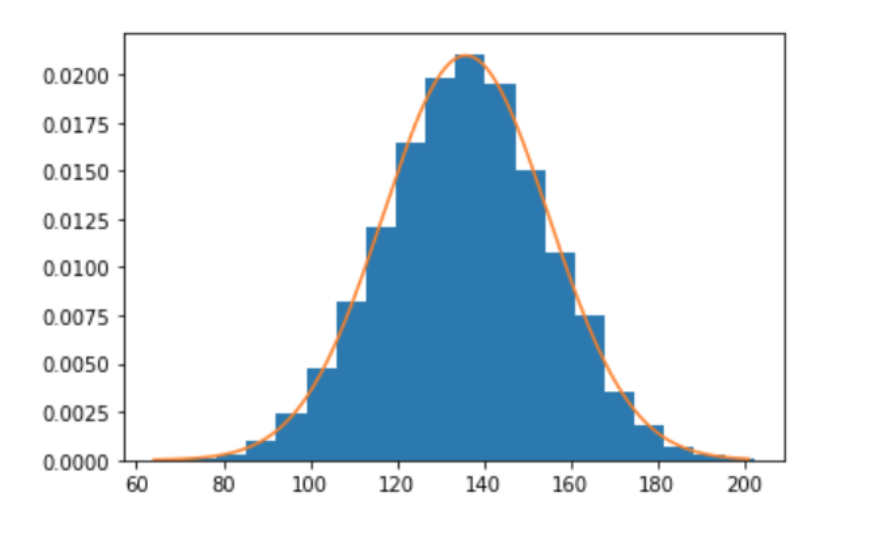
\includegraphics[width=\textwidth]{figs/bins.png}
% 	\caption{An example of approximating a continuous distribution using discrete bins}
% 	\label{fig:binning}
% \end{figure}
	
\section{Conditioning} \label{sec:condition}
	
The GADT described in section \ref{sec:gadt} can be used to describe general models, in particular conditional distributions, thanks to the \texttt{Conditional} variant. Without this variant, we can only define prior distributions, but including it means we can incorporate observed data into our models and perform inference.
	
% https://www.robots.ox.ac.uk/~twgr/assets/pdf/rainforth2017thesis.pdf - section on conditioning, pg.42
The condition variant in my GADT is used to assign scores to traces, and takes a function which takes an element and returns a float, a `score'. This score represents how likely the current trace is, given the value passed to the functions. In this way, we can represent observations.
		
I have also implemented a few helpers to make it easier to condition models. The three main helpers are \texttt{condition}, \texttt{score} and \texttt{observe}, which are all specific cases of the general \texttt{Condition} variant. 
		
The \texttt{condition} operator is used for hard conditioning, which conditions the model on an observation being true. If true is passed in, then the score assigned is 1, and if false, the score assigned is 0. This score represents how likely it is for the current trace to occur, and different inference algorithms will use this information to produce a distribution over all possible traces. We can use this operator to constrain certain variables or outcomes in a model. For example in the below model, we roll two dice and observe that the sum is 4 - we can then find the distribution over the first die (which won't include 4,5 or 6 since they are >=4, the sum).
		
% TODO: put this inline minted (not file) 
% Also not a huge box
% \begin{noindent}
\begin{ocamlcode-in}
let* dice1 = discrete_uniform [1;2;3;4;5;6] in
let* dice2 = discrete_uniform [1;2;3;4;5;6] in
condition (dice1+dice2 = 4)
	(return dice1)
\end{ocamlcode-in}
% \end{noindent}
				
This function is mostly useful for discrete models when using equality in this manner, since the probability of observing any given value in a continuous distribution is zero. However, if we are dealing with ranges, then we can use hard conditioning as in the model below, which constrains the standard normal distribution to be positive.

% TODO: put this inline minted (not file) 
% Also not a huge box
% \begin{noindent}
\begin{ocamlcode-in}
	let* x = normal 0. 1. in
	condition x > 0.
		(return x)		
\end{ocamlcode-in}
% \end{noindent}

For soft conditioning, for example an observation that we know comes from a certain distribution, there is an \texttt{observe} function. This function is essential for continuous distributions, since the probability of observing any one value is 0, making hard conditioning since it will just reject every trace. Instead, we can use the pdf function of the distribution to determine how likely that observation is in the model.

The \texttt{score} function is similar to the condition operator, except instead of 0, it assigns a particular constant score (any float) to the trace. This is generally used in a branch, where a constant score will be assigned depending on some (deterministic) condition.
	
% \begin{noindent}
\begin{listing}[!htb]
	\centering
	\begin{ocamlcode-in}
let condition b d = Conditional((fun _ -> if b then 1. else 0.), d)
let score s d = Conditional((fun _ -> s),d)
let observe x dst d = Conditional((fun _ -> Primitive.pdf dst x),d) 
	\end{ocamlcode-in}	
	\caption{The definitions of the different conditioning operators}
	\label{lst:cond}
\end{listing}
% \end{noindent}
	
\section{Forward Sampling}
% https://www.robots.ox.ac.uk/~twgr/assets/pdf/rainforth2017thesis.pdf - sec 7.1, pg 135
The simplest operation to define on models is to sample from them. Sampling from conditional distributions required inference, and is discussed in section \ref{sec:inference}. Here, we run a probabilistic program 'forwards', that is, running a generative model and seeing the outputs without conditioning on observed data.
		
In PPLs, a complete program can be thought of as a posterior, $P(\theta\mid x)$, the distribution of a parameter given some observed data. The generative model, i.e. the program without condition statements, can be thought of as the prior distribution, $P(\theta)$. The condition statements then define the likelihood model, that is, $P(x\mid \theta)$, the probability of the observations in the current model (the prior). So finding the prior is the same as disregarding the conditionals (essentially ignoring the data). Sampling is only difficult in the presence of conditionals (as this requires inference), so this allows us to sample from the prior using the same sample function defined before. We can also transform any \texttt{'a dist} into a different \texttt{'a dist} that is the prior by ignoring conditional statements.
		
We can also take into account the conditionals, and produce weighted samples, with the weight being the score assigned by each conditional branch, accumulated by multiplying all the scores. This gives us a set of values with corresponding weights which represent how likely those values are. An important property of these weights is that they are not normalised, so we cannot use this to find the posterior directly. I have implemented several variants of functions for finding the prior and sampling, all with the same concept as below.
	
\begin{listing}[!htb]
	\centering
	\ocamlcode{code_snippets/prior_sample.ml}
	\caption{Sampling functions}
	% \label{}
\end{listing}
	
The function for generating a prior does not directly take samples, but manipulates the structure of the dist GADT. For example, in the \texttt{Bind} branch, it actually introduces 2 new bind variants (via \texttt{let*}) which produces a new distribution lazily. This makes it easier to use the prior within inference algorithms, and allows it to be composed with other distribution modifying functions.
	
\section{Inference} \label{sec:inference}
	
Inference is the key motivation behind probabilistic programming. Up to this section, we have discussed how to represent models but not do anything with them that couldn't be done in a standard language. With inference, we can produce a sampler which will accurately reflect a posterior distribution.
	
Inference can be thought of as a program transformation \cite{scibior2015practical} \cite{Zinkov2016ComposingIA}. In my ppl, this corresponds to a function of type \texttt{'a dist -> 'a dist}. This method allows for the composition of inference algorithms, exemplified in section \ref{sec:pimh}.
	
% use equations from here: https://arxiv.org/pdf/1507.00996.pdf
		
% Since I have used a trace-based approach, we can characterise the posterior probability of a trace as (from the previous chapter):
% % https://www.robots.ox.ac.uk/~twgr/assets/pdf/rainforth2017thesis.pdf - pg.52
% $$p(x_{1:N}|y_{1:N})\propto\tilde{p}(y_{1:N},x_{1:N})$$
		
% We can now see how this formula corresponds to a program in my ppl. The example below is a very simple model, which adds two numbers drawn from discrete distributions, and observes a value.
		
% TODO: write example program, and relate to terms in formula
		
\subsection{Enumeration} \label{sec:enum}
Enumeration is the simplest way to perform exact inference on probabilistic programs, and essentially consists of computing the joint distribution over all the random variables in the model. This involves enumerating every execution path in the model, in this case performing a depth first search over the \texttt{dist} data structure. For every \texttt{bind} (i.e. every \texttt{let*}), there is a distribution ($d$) and a function from samples to new distributions ($f$). I call this function on every value in the support of the distribution $d$, and then enumerate all the possibilities. The final output is a \texttt{('a * float) list}, from which duplicates are removed and is then normalised, so that the probabilities sum to one.
		
\begin{listing}[ht]
	\ocamlcode{code_snippets/enumerate.ml}
	\caption{Enumerating all paths through a model}
	\label{lst:enum}
\end{listing}
		
This method is very naive, and therefore inefficient. Since we essentially take every possible execution trace, we do not exploit structure such as overlapping traces. This can be made slightly more efficient by using algorithms such as belief propagation \cite{belief-prop}, but they still only work on models made up from discrete distributions (and are not compatible with the way I represent models). Exact inference of this kind only works on models that can be represented as finite networks, and exact inference for Bayesian networks is in fact NP-hard\cite{cooper1990computational}. So instead, most of my project focuses on approximate inference.
		
\subsection{Rejection Sampling} \label{sec:rej}
% https://www.cs.ubc.ca/~schmidtm/Courses/540-W18/wood.pdf pg30
% Ancestral sampling, very good explanation of rejection
% Why rejection doesn't work for continuous, so must use importance instead -->
% http://www.cs.tut.fi/~elomaa/teach/AI-2013-9.pdf
% Hard rejection
In my implementation of rejection sampling, I take samples from the prior, with accumulated scores. If the score is above some constant threshold, then the sample is accepted, and rejected otherwise. The specific case of the general rejection sampling algorithm used here sets the proposal distribution as the prior, and we use the scores to approximate the density function of the posterior (listing \ref{lst:rej}).
% todo: code of rejection sampling
	
\begin{listing}[!htb]
	\centering
	\ocamlcode{code_snippets/rej.ml}
	\caption{Simplest rejection sampling method}
	\label{lst:rej}
\end{listing}
	
This method is naive, since it runs an entire trace even if the first condition dropped the score below the threshold. An optimisation I implemented is to short-circuit this, and reject as soon as the trace goes below the threshold. This does slightly increase the time taken for small models, and so is not the default. It is also implemented as a dist transformation, so can again be used with the same sample methods.
	
This particular function is hard rejection, since samples with a lower score are always rejected. I have also implemented functionality to perform `soft' rejection. This method instead sets the probability of acceptance being the score attached to the sample.
	
A problem with rejection sampling is if conditions make most execution traces very unlikely. This means it will take a very large number of samples to have enough (or any) accepted samples. An example is given in listing \ref{lst:bad-reject}, where the condition only has a 1\% chance of being true. This means that, on average, for every 1000 samples, we will only accept one.
	
% \begin{noindent}
\begin{listing}[!htb]
	\centering
	\begin{ocamlcode-in}
let* x = bernoulli 0.001 in
condition (x=0)
(return x)
	\end{ocamlcode-in}
		
	\caption{An example of a model that is very inefficient under rejection sampling}
	\label{lst:bad-reject}
\end{listing}
% \end{noindent}
% 
\subsection{Likelihood Weighting} \label{sec:likelihood-wighting}
% http://www.cs.tut.fi/~elomaa/teach/AI-2013-9.pdf
		
Likelihood weighting is an importance sampling method, when the proposal distribution we use is the prior. We want any algorithm we use to be as general as possible, and not need to be tuned using auxiliary distributions chosen by hand. Since for any model we can find the prior distribution easily, it is natural to use this as a proposal distribution here - this can be seen in several of the implementations of inference. 
	
The implementation of likelihood weighting is simple - we simply take a set of samples (with weights) from the prior, remove duplicates and normalise, and use this set of particles as a the categorical distribution representing the posterior.
% \begin{noindent}	
	\begin{listing}[!htb]
		\centering
		\begin{ocamlcode-in}
let importance n d = 
let particles_dist = sequence @@ List.init n ~f:(fun _ -> prior d) in
let* particles = particles_dist in 
categorical particles
		\end{ocamlcode-in}
		\caption{Likelihood weighting}
		\label{lst:imp}
	\end{listing}
% \end{noindent}
	
The sequence function is a monad function that takes a list of distributions and fold them together so that they act as a single distribution returning entire lists. This allows The use of \texttt{(let*)} to sample a set of particles at once, and use them directly as the distribution.
% code of importance sampling.
	
\subsection{Metropolis Hastings} \label{sec:mh}
Metropolis Hastings is an MCMC algorithm, and so is used to find a Markov chain with the stationary distribution equal to the target distribution, here the posterior. There are many variants of this algorithm, and the one I implement here is the independent metropolis hastings (IMH) algorithm. I use the prior as a proposal distribution, using scores as an approximation to a density function. The algorithm is outlined below.
\begin{itemize}
	\item Let $\pi$ be the target distribution that we want to sample from.
	\item Let $q$ be the density function of the prior, approximated by the scores.
	\item Initialise by taking a sample from the prior as the first state in the chain.
	\item Let x be a sample from the prior.
	\item Let y be the last state in the chain.
	\item Calculate the acceptance probability, $\alpha(x,y)$ by \eqref{eq:accept}
	      \begin{equation}
	      	\label{eq:accept}
	      	\alpha(x,y) = 
	      	\begin{cases}	
	      		\min{\left( \frac{\pi(y)q(x)}{\pi{x}q(y)},1 \right) } & \pi(x)q(x) > 0 \\
	      		1                                                     & \pi(x)q(x) = 0 \\
	      	\end{cases}
	      \end{equation}	      	      	      	      
	\item The state x is then accepted with probability $\alpha(x,y)$. If accepted, we use x as the next state, or if rejected, we re-use y as the next state. 
\end{itemize}
	
This produces a Markov chain with transition probability: \[p(x, y) = q(y)\alpha(x, y) \quad\quad y\neq x\].
It is known as `independent' metropolis hastings since subsequent candidate states ($x$) are independent on previous values of states.
	
% https://probmods.org/chapters/inference-algorithms.html
% MCMC section
I have implemented IMH as a function transforming \texttt{'a dist}s (\texttt{'a dist -> 'a dist}). This allows it to be composed with other inference algorithms, as well as allowing the standard sample function to be used on the output. To model a Markov chain, I use a \texttt{Core.Sequence}, which is a data structure for a lazy list. The creator function uses a function that takes a previous state to produce a new state and output a value - analogous to the transition function. In this case, the output is the same as the state.
	
One important property of the return distribution is that consecutive sample statements will need to return different values (to simulate running the chain). In order to achieve this, I create some mutable state - the sequence, which will take a step every time sample is called on the output distribution. In order to make sure this sequence is persistent, I use a reference and put it after a bind (let*) statement, incrementing the chain every time the function is called (which is only on sampling). Since the bind statement contains a function, the reference is closed over and is persistent to the output distribution.
	
\begin{listing}[!htb]
	\centering
	\ocamlcode{code_snippets/mh.ml}
	\caption{Metropolis hastings}
	\label{lst:mh}
\end{listing}
	
\subsection{Bootstrap Particle Filter} \label{sec:pf}
% https://probmods.org/chapters/inference-algorithms.html
% particle filter section
Particle Filters are a class of algorithms which use particles to approximate a posterior. This is similar to the technique I used in importance sampling (\ref{sec:likelihood-wighting}), but the difference here is that the particles are sequentially updated as we observe condition statements (i.e. as we observe data). In fact, an example of a particle filtering algorithm is sequential importance sampling, but here I use an algorithm called the bootstrap filter \cite{particlefilter}.
	
The code given in listing \ref{lst:smc} transforms a conditional distribution to a new conditional distribution. In order to find the posterior, we simply ignore the conditional by finding the prior after using the smc method.
	
\begin{listing}[!htb]
	\centering
	\ocamlcode{code_snippets/smc.ml}
	\caption{Particle Filter}
	\label{lst:smc}
\end{listing}
	
The GADT is traversed top down, with particles being initialised at a `leaf' - primitives or returns. From this root, bind functions apply functions to the particles, and conditional statements updates the weights and resamples. The \texttt{resample} function takes a set of particles and takes samples from this set with replacement - this is the `bootstrap' resampling method. The output distribution is conditioned by the total weight of all particles.
	
Increasing the number of particles finds a more accurate distribution, but also increases the amount of time and memory required.
	
\subsection{Particle Cascade} \label{sec:pc}
The particle cascade algorithm (also Asynchronous Sequential Monte-Carlo) is an algorithm that extends the particle filter, introduced in (Paige et al. 2014) \cite{paige2014asynchronous}. It uses a lazily generated infinite set of particles, which allows it to be `anytime', that is, it can generate more particles without having to start regenerate a large particle set from scratch. It also features a parallelisable re-sample step, although I will not make use of this feature, since I am not using multi-core OCaml.
	
The main implementation difference is that instead of resampling, a particle `branching' operation is used, which produces a lazily generated set of particles at each resample step. Each particle produces 0 or more children to be used in the next iteration.
	
\subsection{Particle-Independent Metropolis-Hastings} \label{sec:pimh}
	
SMC and MCMC algorithms are two distinct classes of algorithms, but can be combined to produce more efficient inference procedures. A simple example of these algorithms (known as PMCMC), is the particle-independent metropolis-hastings algorithm \cite{pmcmc}. This algorithm first uses a particle filter to find an approximation of the posterior, then uses this approximation as a prior distribution for metropolis-hastings.
	
% TODO: describe maths using https://www.maths.lancs.ac.uk/~sherlocc/CompStats/Dawn_of_Time/PseudoMarg/compstats_PIMH_BT.pdf
	
Due to the fact that my PPL allows composition of inference algorithms, a basic implementation is very simple.
	
% \begin{noindent}
	\begin{ocamlcode-in}
let pimh k n d = mh k (Smc.smc n d)
	\end{ocamlcode-in}
% \end{noindent}
However, there are flaws in this implementation, since any sampler produced is slow and can be made more efficient.
In addition, the reason this works is because the \texttt{smc} function produces a dist with conditionals, which no other inference method does.
	
% These examples should really be in evaluation
\section{Visualisations}
Visualising the output distributions from inference can be done using the \texttt{Owl\_plplot} module, which allows plotting directly from OCaml, rather than having to interface with other programs manually. I have implemented several helper functions which simplify visualising distributions created by my PPL. Empirical distributions are approximated by histograms displayed as bar charts using \texttt{Owl\_plplot}.
	
For discrete distributions, this conversion is simple - each bar is simply the pmf (probability mass function) of the distribution at each value in the support. This is calculated by drawing $N$ samples, then for each value $x_i$, finding $\frac{n}{N}$, where $n$ is the number of samples that equal $x_i$, to find the approximate probability of that value in the distribution, $P(X = x_i)$.
	
Where there is an ordering on the type, discrete distributions can also have their cdf visualised. The cdf of a discrete distribution is a step function. The ordering is given by a first class module representing the type. There are cases where there is no natural ordering - for example a distribution over an arbitrary ADT, so this also allows a user to custom define the ordering.
% 
\begin{figure}[!htb]
	\centering
	\subfloat[PDF]{{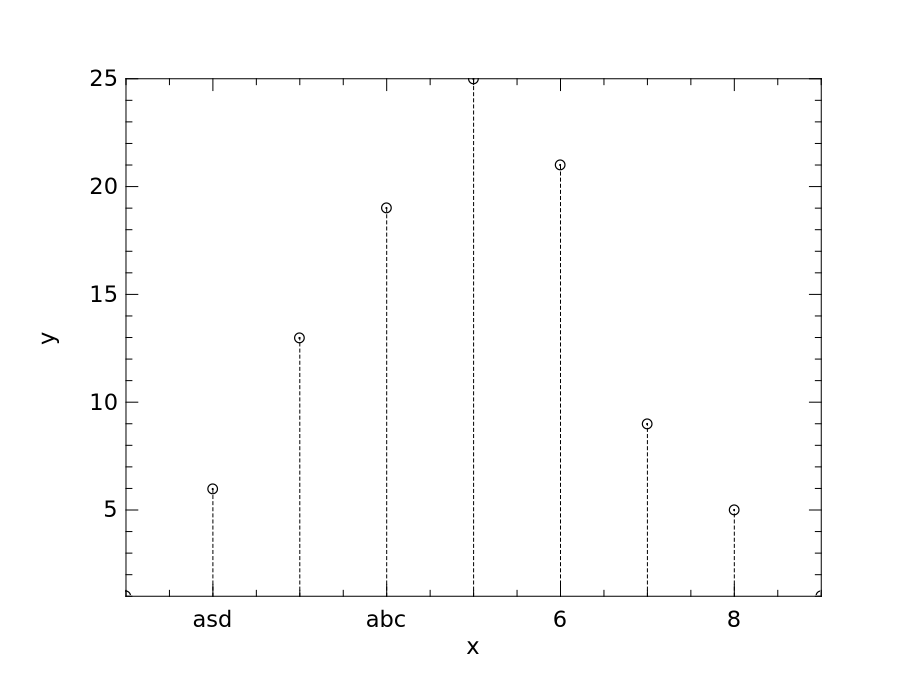
\includegraphics[width=0.4\textwidth]{figs/binompdf_hist.png} }}%
	\qquad
	\subfloat[CDF]{{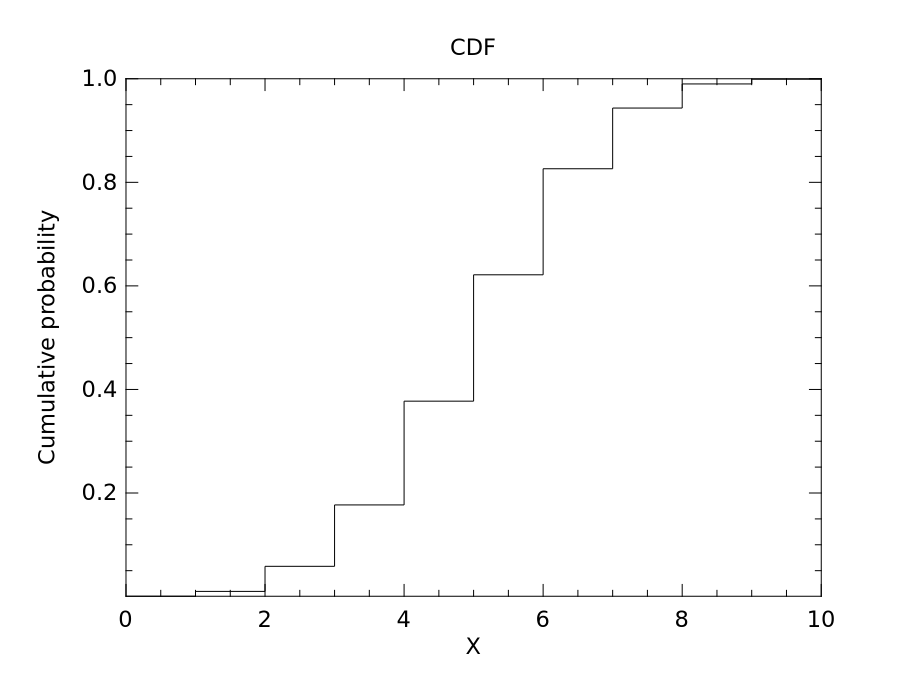
\includegraphics[width=0.4\textwidth]{figs/binom_ecdf.png} }}%
	\caption{Samples from a binomial distribution visualised, $n=10,000$}
	\label{fig:vis-binom}
\end{figure}
% 
Continuous distributions are also displayed as histograms, with a set of samples being put into $n$ equal width bins. The height of each bar is the the pdf (continuous analogue to the pmf), which is calculated by finding the number of samples in each bin, then dividing by the total number of samples. To display the cdf, we can display the empirical cdf directly as a scatter plot, or join points to draw a step function.
	
\begin{figure}[!htb]
	\centering
	\subfloat[PDF]{{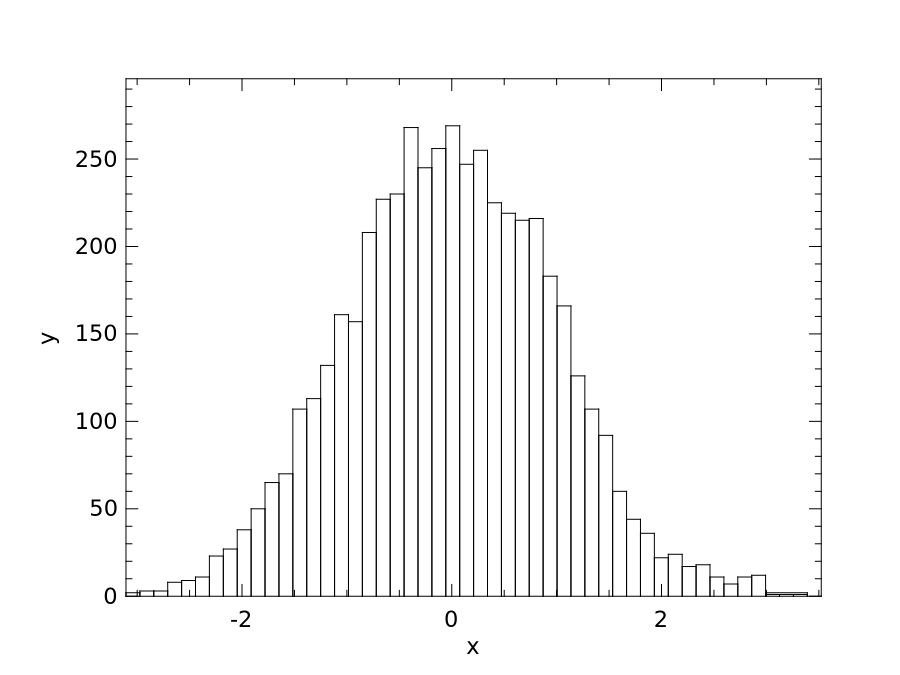
\includegraphics[width=0.4\textwidth]{figs/normpdf_hist.png} }}%
	\qquad
	\subfloat[CDF]{{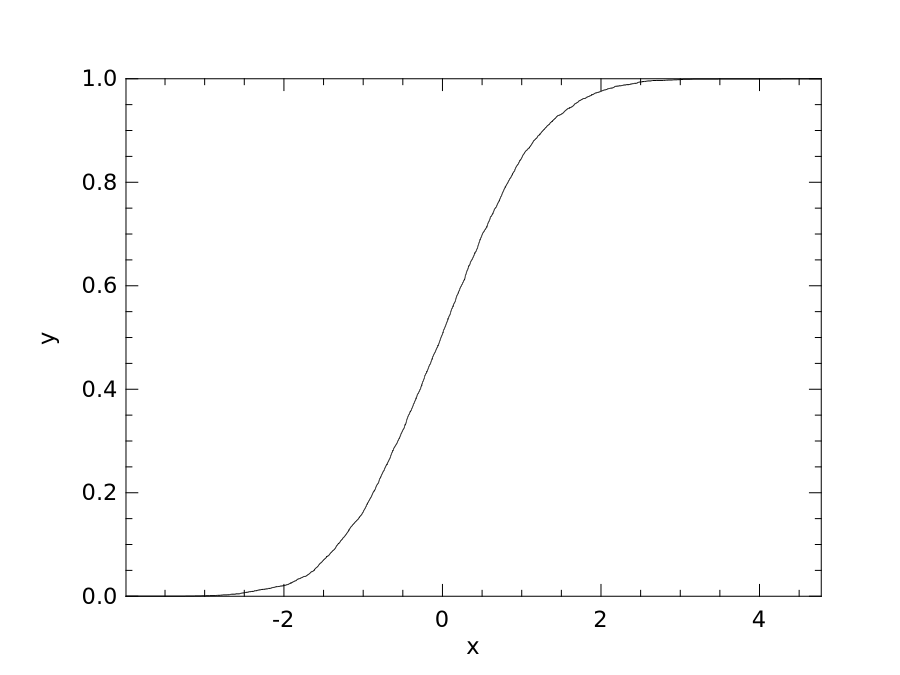
\includegraphics[width=0.4\textwidth]{figs/norm_ecdf.png} }}%
	\caption{Approximate pdf and cdf of samples from a standard normal distribution}
	\label{fig:vis-norm}
\end{figure}
	
Other important visualisations for continuous distributions are the Q-Q and P-P plots. These provides a way to qualitatively compare distributions. P-P plots plot the cdfs of two distributions against each other, that is, for two cdfs $F$ and $G$, the points $(F(z), G(z))$ are plotted for some values of z in the range $(-\infty,+\infty)$. Q-Q plots plot the quantiles of both distributions - it uses the inverse of the cdfs (the ppf) to plot the points $(F^{-1}(q), G^{-1}(q))$, where $q$, the quantile, is in the interval $[0,1]$. This plots will generally use as many points as the data allows, and calculate the percentile for every data point available. For both plots, if all the points lie on the the line $y=x$, the distributions are identical. These plots are often used to find the differences between some theoretical expected distribution and the distribution given by some data. This can be used in the PPL context to find whether a distribution given by a model matches what was expected in the theory. Figure \ref{fig:vis-qq} shows the output of inference for a model that is expected to output a beta distributions (the coin model in section \ref{sec:coin}) - the points are close to the expected line, showing successful inference.

\begin{figure}[!htb]
	\centering
	\subfloat[Q-Q plot]{{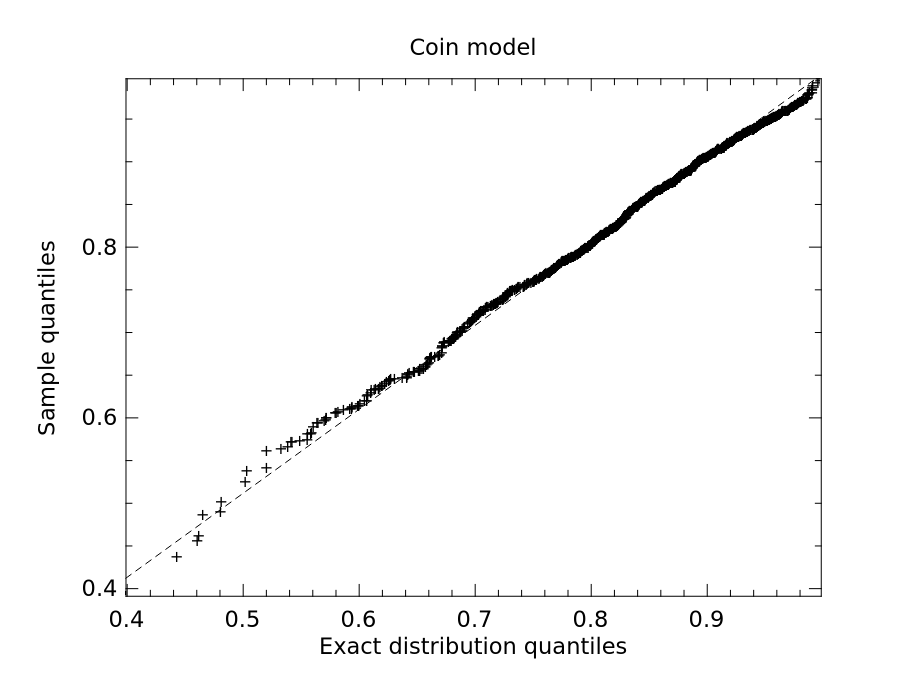
\includegraphics[width=0.4\textwidth]{figs/qq.png} }}%
	\qquad
	\subfloat[P-P plot]{{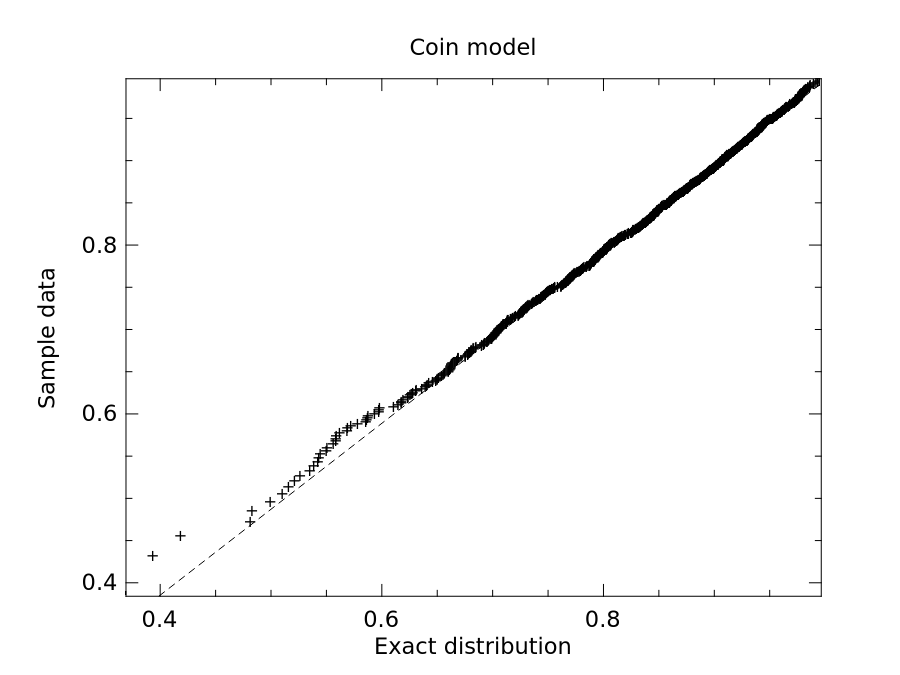
\includegraphics[width=0.4\textwidth]{figs/pp.png} }}%
	\caption{Plots to compare inferred distributions with the exact solutions}
	\label{fig:vis-qq}
\end{figure}
	
For primitive continuous distributions, a smooth line can also be drawn since we have a function that can calculate the exact pdf or cdf. This can also be overlaid onto a histogram, to again compare two distributions. Figure \ref{fig:vis-samples} shows an exact beta distribution overlaid onto samples taken from the inferred distribution.
	
\begin{figure}[!htb]
	\centering														
	\begin{minipage}{0.45\textwidth}
		\centering
		\ocamlcode{code_snippets/plotter.ml}
		% \captionof{listing}{Code to produce plot}
	\end{minipage}
	\begin{minipage}{0.45\textwidth}
		\centering
		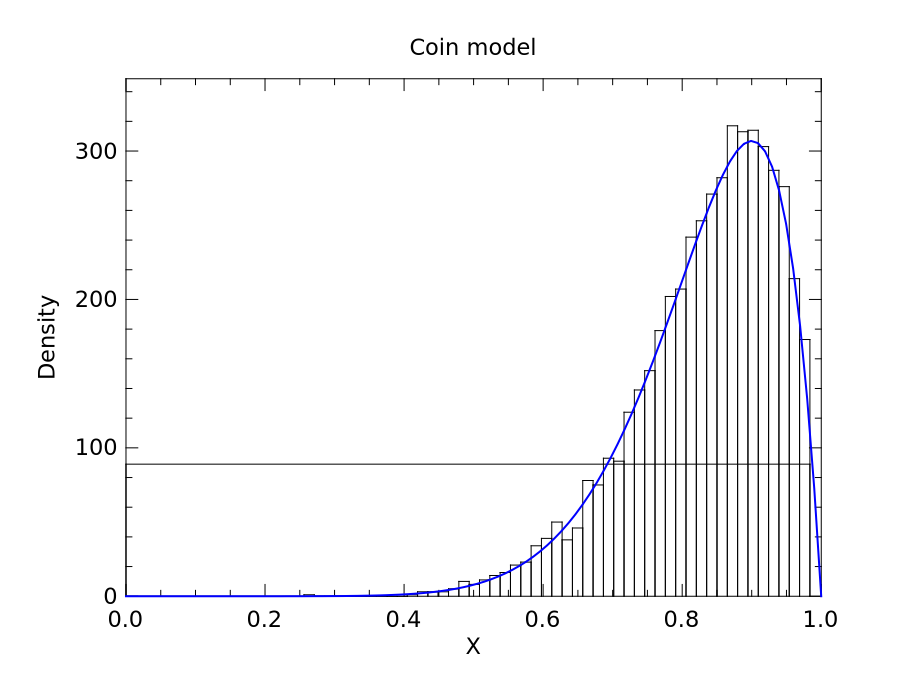
\includegraphics[width=\linewidth]{figs/coin_compare.png}
		% \captionof{figure}{Output}
	\end{minipage}
	% 
	\caption{The approximate and exact pdf of the output of inference for a biased coin model, with code to produce plot}
	\label{fig:vis-samples}
\end{figure}
	
	
\section{Testing}
	
Automated testing of PPLs is difficult for reasons outlined in section \ref{sec:prep-testing}. However, I still wrote basic unit tests. The test framework I used, Alcotest, lets me check that outputs of functions match expected values. This allows me to test all deterministic helper functions, e.g. normalise. It also lets me test the exact inference method, and very simple distributions and models which only contain a single value. I also used an additional library Quickcheck, to test that a specified invariant holds for a function - it uses randomly generated inputs to check the widest range of values. As an example (listing \ref{lst:test}), for the normalise function, we expect that the output probabilities always sum to one, no matter the input array - the test is given below.
	
	
% \begin{noindent}
\begin{listing}[!htb]
	\centering
	\begin{ocamlcode-in} 
let test_normalise_sum_to_1 =
QCheck.Test.make ~count:1000 ~name:"test normalisation"
QCheck.(list (pair int float)) (* type to randomly generate *)
(fun l -> (List.sum ~f:snd (normalise l)) = 1.)
	\end{ocamlcode-in}
	\caption{Testing the normalisation function for particles}
	\label{lst:test}
\end{listing}
% \end{noindent}
	
The test output and code coverage output can be seen in figure \ref{fig:test-out}.
\begin{figure}[!htb]
	\centering
	\subfloat[Test report, abbreviated]{{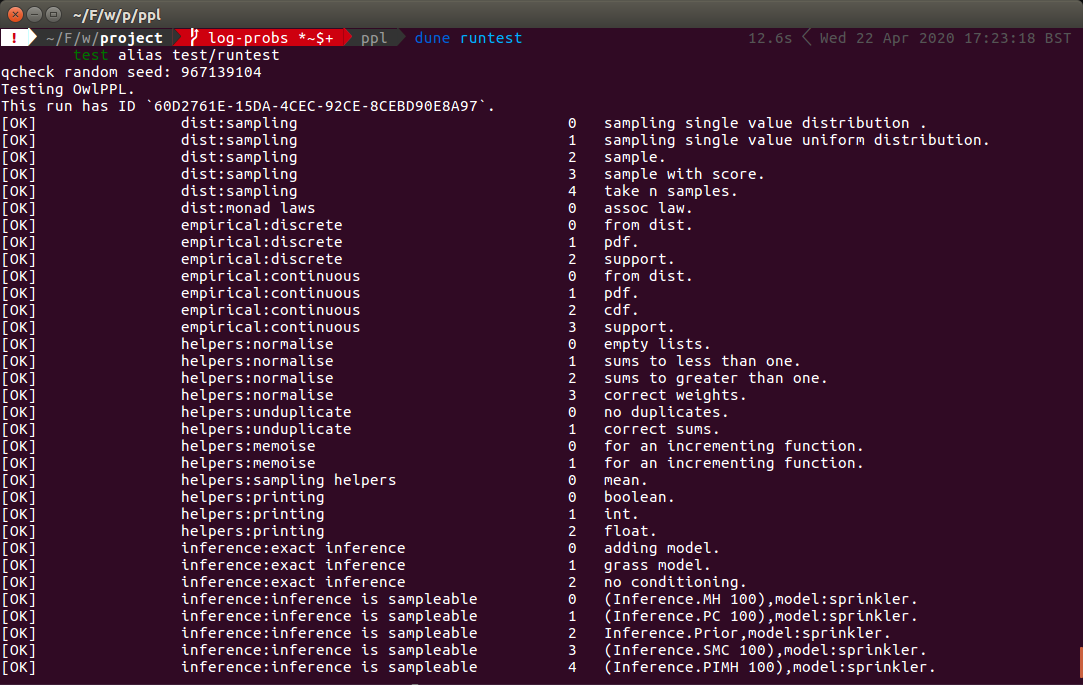
\includegraphics[width=\textwidth]{figs/tests.png} }}%
	\qquad
	\subfloat[Code coverage report]{{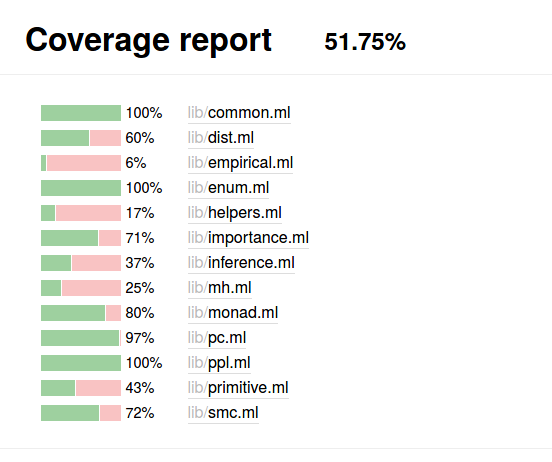
\includegraphics[width=0.6\textwidth]{figs/coverage.png} }}%
	\caption{Output from running unit tests}
	\label{fig:test-out}
\end{figure}
% !TeX root = ../diss.tex

% sketch out what plots to include here
% - plot of kl divergence w.r.t. number of samples taken
% - plot of running time w.r.t. amount of data conditioned on
% - plot of running time w.r.t. number of particles (for smc)
% - maximum memory footprint (against parameters as above)
% - total memory footprint over time
% box plots instead of just lines

% use ppl to do evaluation? good to show code in my language which does evaluation

% explain WHY in evaluation, how just what - e.g. explain why plot looks how it does, don't just describe

% show some output from merlin to show the fact that type inference works and is good?
So far, I have developed a PPL that can be used to define arbitrary probabilistic models and perform Bayesian inference on them. To evaluate the performance of my PPL, I will present some examples to show programs written in my PPL translated into equivalent programs in other PPLs, and then measure time and memory consumption of inference\footnote{All tests are carried out on a single core of an Intel\textsuperscript{(R)} Core\textsuperscript{(TM)} i5-7200U CPU @ 2.50GHz}. I will also determine the correctness of inference procedures by using hypothesis tests which use drawn samples to determine whether two distributions are the same or not.

\section{Examples}
To show how my PPL would be used on real problems, I now outline a set of example problems. Several examples here will be simple, and have analytic solutions - this is so that I can then test the correctness of applying inference on them. More complex realistic models are also included to test performance. Full derivations of the solutions as well as mathematical descriptions of the models are given in appendix \ref{app:examples}.

\subsection{Sprinkler}
% to show exact inference on discrete model
The sprinkler model is a commonly used example in Bayesian inference due to it's simplicity. It is an example of a \textit{Bayesian network}, and can be visualised as in figure \ref{fig:sprinkler-network}. The code in listing \ref{lst:sprinkler} shows the model in the diagram encoded as a program. This particular program can be used (by applying an inference function) to find the probability of rain given that the grass is wet.
	

\begin{listing}[!ht]
	\ocamlcode{code_snippets/sprinkler.ml}	
	\caption{Sprinkler model}
	\label{lst:sprinkler}
\end{listing}

\begin{figure}[!htb]
	\centering
	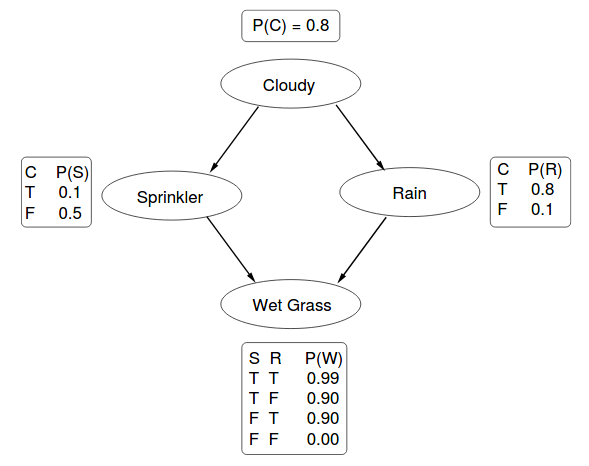
\includegraphics[width=0.5\textwidth]{figs/sprinkler-network.png}
	\caption{Bayesian Network example}
	\label{fig:sprinkler-network}
\end{figure}

\subsection{Biased Coin} \label{sec:coin} 
% to show analytically solvable continuous distribution
% include graph of beta compared to computed posterior
Modelling a biased coin shows an example of a very simple model with a continuous posterior that can be calculated analytically\cite{datasci}. 
% 
The model is of a coin that is tossed $n$ times to give $x$ heads. We do not know if the coin is biased or not, and would like to find out the bias, $p$ of the coin, where $p$ is the probability of heads, with $p=0.5$ being an unbiased coin.
% 
To find the posterior, we use an uninformative prior ($\Theta$), the uniform. This results in the posterior, the beta distribution, specifically Beta$(x+1,n-x+1)$.

The program in my PPL is shown in listing \ref{lst:coin}, and demonstrates setting up the model, performing inference as well as finding the mean of the posterior. The application is to find the chance of the next coin flip landing heads. This example uses $n=10$ and $x=9$, so the mean produced is roughly 0.83, the mean of Beta$(10,2)$.

\begin{listing}[!ht]
	\ocamlcode{code_snippets/coin.ml}	
	\caption{Coin model}
	\label{lst:coin}
\end{listing}

\begin{figure}[!htb]
	\begin{minipage}{0.5\textwidth}
		\centering
		\jscode{code_snippets/webppl/coin.js}
		\captionof{listing}{WebPPL}
	\end{minipage}
	\begin{minipage}{0.5\textwidth}
		\centering
		\clojurecode{code_snippets/anglican/coin.clj}
		\captionof{listing}{Anglican}
	\end{minipage}
	\caption{The coin model in WebPPL (JS) and Anglican (Clojure)}
	\label{fig:compare-coin}
\end{figure}

The comparison given in Figure \ref{fig:compare-coin} shows how the same model is defined in other languages. Both languages use similar constructs, despite differing syntax. This example also shows that my PPL is similar to existing systems, and is not more verbose.

\subsection{HMM}
Hidden Markov models are slightly more involved models, where we have a sequence of hidden states, which emit observed states. There are two distributions involved here, the transition distribution, which defines how likely the next state is given the current state, and the emission distribution, which is the distribution over the observed states given the hidden state. The example in Listing \ref{lst:hmm} uses discrete distributions, but any type of distribution can be used. The exact posterior for simple models can be found using the forward-backward algorithm.
% use forward-backward to get exact posterior
\begin{listing}[!ht]
	\ocamlcode{code_snippets/hmm.ml}
	\caption{Hidden Markov Model}
	\label{lst:hmm}
\end{listing}

\subsection{Linear Regression}
This example shows how to use multiple data points to infer a continuous distribution. This example can be used to infer the parameters of a line through a set of 2-D points. The fold function can be used to condition on many observations easily. The fmap function is used to map outputs from a distribution. Since the linreg model produces tuples of parameters, we can create individual distributions over either one.

\begin{listing}[!ht]
	\ocamlcode{code_snippets/linreg.ml}	
	\caption{Linear Regression}
	\label{lst:linreg}
\end{listing}

\subsection{Infinite Mixture Model}
This example demonstrates a model which cannot be expressed in some PPLs such as STAN or Infer.Net, since it is a non-parametric Bayesian model. This is a Dirichlet Process mixture model with an infinite number of Gaussians\cite{dpmm}. It is used for the common task of clustering a set of data points without knowledge of the number of clusters. This means the number of clusters is allowed to grow with the dataset size. We use a mixture of Gaussians, meaning the likelihood of a point belonging to each cluster is given by different normal distributions. The full code for this model, along with comparisons to other languages is given in appendix \ref{app:dp}.
% Need to show examples which can't be done in graph based thing
% Need to explain why these examples are actually difficult.
% http://www.cs.cmu.edu/~epxing/Class/10708-16/slide/lecture18-DP.pdf
% This is a non-parametric Bayesian model - 
% no. of params is infinite, grows with size of dataset


\section{Statistical tests}
To evaluate the correctness of my PPL, I used statistical tests which measure goodness-of-fit, i.e. how similar two distributions are to each other. I compare the empirical distribution of 10,000 samples from an approximated distribution to an exact distribution which is calculated analytically. Test statistic distributions (e.g. the $\chi^2$ distribution) were calculated using \texttt{Owl}, and empirical distributions generated using the \texttt{EmpiricalDist} modules.

For all tests described below, I set the significance level, $\alpha = 0.05$ and use null and alternative hypotheses as follows:

$H_0:$ The sample data follow the exact distribution\\
$H_1:$ The sample data do not follow the exact distribution

\subsection{Chi-squared}

The $\chi^2$ test is a simple goodness-of-fit test which can test whether or not a given discrete distribution 

The test statistic is as follows, with each $i$ being a distinct element in the distribution, $x_i$ is the observed number of samples with the value $i$, and $m_i$ is the expected number of samples for the value $i$.

$$X^{2}=\sum _{i=1}^{k}{\frac {(x_{i}-m_{i})^{2}}{m_{i}}}$$

This test statistic is compared against the critical value (at the significance level) of the chi-squared distribution, with the degrees of freedom being $k-1$, where k is the number of possible values of the distribution.
\subsubsection{Results}
\begin{table}[!ht]
	\centering
	\csvautotabular{data/hypothesis-chi.csv}
	\caption{p-values of $\chi^2$ test on different models using different inference procedures}
	\label{tab:chi-pvals}
\end{table}

Table \ref{tab:chi-pvals} shows the results of carrying out the test on several inference procedures for different discrete models. None of the values are below 0.05, so we cannot reject the null hypothesis, so we conclude that, at the 5\% significance level, the distributions are not significantly different.

\subsection{Kolmogorov-Smirnov}

The Kolmogorov-Smirnov test is a non parametric test which is used to compare a set of samples with a distribution - this is the one-sample K-S test. There is also a two-sample K-S test, which compares two sets of samples against each other. I use the one-sample test here to compare samples taken from the inferred posteriors to their exact analytic solutions.

The test statistic is as follows, with $F_n(x)$ being the empirical cumulative distribution of n samples, and $F(x)$ being the exact cumulative distribution.
\begin{align*}
	F_{n}(x) & =\frac{1}{n}\sum_{i=1}^{n}I_{[-\infty ,x]}(X_{i}) \\
	D_{n}    & =\sup_{x}|F_{n}(x)-F(x)|                          
\end{align*}
This test statistic is compared against the critical values of the Kolmogorov distribution, rejecting the null hypothesis if $\sqrt{n}D_n > K_\alpha$, where $K_\alpha$ is the critical value at the significance level $\alpha$, and $n$ is the number of samples.

\subsubsection{Results}

Table \ref{tab:ks-pvals} shows that for all the continuous models considered, the p-value obtained from all tests are greater than then 0.05. This means we do not reject $H_0$ for any model/inference procedure combination, so can be confident (at the 5\% significance level) that the inference procedures are correct. This shows that the generated posterior is not significantly different from the real solution.

\begin{table}[!ht]
	\centering
	% \begin{tabular}{|l|l|l|l|l|}
	% 	\hline
	% 	            & rejection & importance & metropolis-hastings & particle filter \\ \hline
	% 	single coin &           &            &                     &                 \\ \hline
	% 	hmm         &           &            &                     &                 \\ \hline
	% \end{tabular}
	\csvautotabular{data/hypothesis-ks.csv}
	\caption{p-values of K-S test on different models using different inference procedures}
	\label{tab:ks-pvals}
\end{table}


\section{Convergence of sampling}
% TODO: add a few lines to show difference between 
I also used the KL-divergence metric to determine the (dis)similarity of two distributions. The formula for KL Divergence of discrete distributions $P$ and $Q$ is easy to calculate by \eqref{eq:kl_disc}

$${D_{\text{KL}}(P\parallel Q)=\sum _{x\in {\mathcal {X}}}P(x)\log \left({\frac {P(x)}{Q(x)}}\right)}$$ \label{eq:kl_disc}

The continuous version is similar, with $p$ and $q$ now being density functions as in \eqref{eq:kl_cont}. 

$${D_\text{KL}}(P\parallel Q)=\int _{-\infty }^{\infty }p(x)\log \left({\frac {p(x)}{q(x)}}\right)\,dx$$ \label{eq:kl_cont}

% Since we cannot compute this integral exactly (we only have the exact density function for one of the distributions), I put the set of samples into discrete bins to approximate $q(x)$. I then used Monte Carlo integration to compute the integral. 
Since I only have a set of samples from $q$, this integral can't be calculated exactly - there is no exact density function. However, there are ways to estimate density functions, as in (Perez 2008) \cite{perez2008kullback}. The first step is to approximate the cdf by finding the empirical cdf ($P_e$) then linearly interpolating between points to produce a continuous function ($P_c$). Estimating the derivative of $P_c$ then gives the pdf, $\hat{P}$. The final estimator \eqref{eq:final_kl_est} is given by using the exact pdf of $q$ and performing Monte Carlo integration.

\begin{gather}
	P_e(x) = \frac1{n}\sum_{i=1}^n U(x-x_i)\text{ where U is the step function}\\
	P_c(x) = \begin{cases}
	0    & x<x_0                  \\
	a_ix+b_i & x_{i-1} \leq x \le x_i \\
	1    & x_{n+1} \leq x         
	\end{cases}\\
	\hat{P}(x) = \frac{P_c(x+\delta) - P_c(x)}{\delta} \text{ for sufficiently small }\delta\\
	\hat{D}_{KL}(P \| Q) = \frac1{n}\sum_{i=1}^n \log\left(\frac{\hat{P}(x_i)}{q(x_i)}\right)\\ \label{eq:final_kl_est}
\end{gather}
% 
Both the metrics (discrete and continuous) were computed with code written using the \texttt{EmpiricalDist} modules.

The idea behind conducting this test is ensuring that the KL divergence decreases as we take more samples from the posterior. This ensures that the solution converges to the correct distribution - a KL divergence of 0 implies the distributions are identical.

Figure \ref{fig:kl} shows the results of this. For each inference procedure, we can see that the KL-divergence for each model decreases as we take more samples. In the case of the sprinkler model, there is a rise near the end, but this can be attributed to noise since the KL-divergence is actually lowest for that model, implying that inference performed best for it.

\begin{figure}[!ht]
	\centering
	\begin{tikzpicture}
		\pgfplotstableread[col sep = comma]{data/kl/kl_coin_all.csv}\datatable
		\pgfplotstablegetcolsof{\datatable}
		\pgfmathtruncatemacro\numberofcols{\pgfplotsretval-1}
		\begin{loglogaxis}[
				title={Coin model}, 
				xlabel={number of samples}, 
				ylabel={KL divergence},
				width=0.45\textwidth,
				legend style={at={(0.5,-0.28)},
					anchor=north,legend columns=-1}
			]
			\addplot table [x index=0, y index=1, col sep=comma] {data/kl/coin_mh.csv};
			\addlegendentry{mh}
			% 
			% \addplot table [x index=0, y index=1, col sep=comma] {data/kl/coin_rej.csv};
			% \addlegendentry{rejection}
			% 
			\addplot table [x index=0, y index=1, col sep=comma] {data/kl/coin_imp.csv};
			\addlegendentry{importance}
			% 
			\addplot table [x index=0, y index=1, col sep=comma] {data/kl/coin_smc.csv};
			\addlegendentry{smc}
			% 
			% \pgfplotsinvokeforeach{1,...,\numberofcols}{
			% 	\addplot table [x index=0,y index=#1, col sep=comma] {data/kl/kl_coin_all.csv};
			% 	\pgfplotstablegetcolumnnamebyindex{#1}\of{\datatable}\to{\colname}
			% 	\addlegendentryexpanded{\colname}
			% }
		\end{loglogaxis}
	\end{tikzpicture}
	\begin{tikzpicture}
		\pgfplotstableread[col sep = comma]{data/kl/kl_sprinkler_all.csv}\datatable
		\pgfplotstablegetcolsof{\datatable}
		\pgfmathtruncatemacro\numberofcols{\pgfplotsretval-1}
		\begin{loglogaxis}[
				title={Sprinkler model}, 
				xlabel={number of samples}, 
				ylabel={KL divergence},
				width=0.45\textwidth,
				legend style={at={(0.5,-0.28)},
					anchor=north,legend columns=-1}
			]
			\addplot table [x index=0, y index=1, col sep=comma] {data/kl/sprinkler_mh.csv};
			\addlegendentry{mh}
			% 
			% \addplot table [x index=0, y index=1, col sep=comma] {data/kl/sprinkler_rej.csv};
			% \addlegendentry{rejection}
			% 
			\addplot table [x index=0, y index=1, col sep=comma] {data/kl/sprinkler_imp.csv};
			\addlegendentry{importance}
			% 
			\addplot table [x index=0, y index=1, col sep=comma] {data/kl/sprinkler_smc.csv};
			\addlegendentry{smc}
			% 
																																																																																																																																																																																																																																																																																																						
			% \pgfplotsinvokeforeach{1,...,\numberofcols}{
			% 	\addplot table [x index=0,y index=#1, col sep=comma] {data/kl/kl_sprinkler_all.csv};
			% 	\pgfplotstablegetcolumnnamebyindex{#1}\of{\datatable}\to{\colname}
			% 	\addlegendentryexpanded{\colname}
			% }
		\end{loglogaxis}
	\end{tikzpicture}
	\caption{Plot of KL-divergence with increasing number of samples for different models and inference procedures}
	\label{fig:kl}
\end{figure}


\section{Performance}
% probabilistic c (paige14) makes the same comparison
% TODO: measure performance with varying no. particles (measure KL with difference no. particles)

I evaluated the performance of my ppl against Anglican, WebPPL, and Pyro. All of these languages are universal PPLs embedded in different host languages, so are comparable to my PPL.

Figures \ref{fig:time-perf} and \ref{fig:mem-perf} shows how my PPL compares against these languages for a range of models and inference procedures. All the models have been introduced previously, and have been shown to produce correct results in my PPL when using the given inference procedures. I measure both running time and peak memory usage.

\newcommand{\perfgraph}[3]{
	\begin{tikzpicture}
		\pgfplotstableread[col sep = comma]{#1}\datatable
		\pgfplotstablegetcolsof{\datatable}
		\pgfmathtruncatemacro\numberofcols{(\pgfplotsretval-1)*0.5}
		\begin{axis}[
				ylabel={#3},
				ymin=0,
				legend style={at={(0.5,-0.15)},
					anchor=north,legend columns=-1},
				ybar,
				xtick=data,
				xticklabels from table={\datatable}{model},
				title={#2},
				width=0.45\textwidth
			]
			\pgfplotsinvokeforeach{1,...,\numberofcols}{
				\pgfmathtruncatemacro\e{##1 + \numberofcols}
				\pgfplotstablegetcolumnnamebyindex{##1}\of{\datatable}\to{\colname}
				\addplot+[error bars/.cd, y dir=both, y explicit,  error bar style={color=black}] table [x expr=\coordindex,y index=##1, col sep=comma, y error index=\e] {#1};
				\addlegendentryexpanded{\colname}
			}
		\end{axis}
	\end{tikzpicture}%
}
			
\begin{figure}[!ht]
	\centering
	% \perfgraph{data/times_mh.csv}{Metropolis-Hastings}{time (ms)}
	% \perfgraph{data/times_smc.csv}{Particle Filter}{time (ms)}
	% \perfgraph{data/times_rej.csv}{Rejection Sampling}{time (ms)}
																																															
	\perfgraph{data/times_coin.csv}{Biased Coin}{time (ms)}
	\perfgraph{data/times_linreg.csv}{Linear Regression}{time (ms)}
	\perfgraph{data/times_hmm.csv}{Hidden Markov Model}{time (ms)}
	\perfgraph{data/times_sprinkler.csv}{Sprinkler}{time (ms)}
																																															
	\caption{Performance of my ppl against other languages for different models and inference algorithms, taking 10,000 samples from the posterior, averaged over 20 runs. Error bars show the 95\% confidence interval}
	\label{fig:time-perf}
\end{figure}
			
\begin{figure}[!ht]
	\centering
	% TODO: ADD ERROR BARS for maybe 95% confidence interval - use ppl to generate confidence interval 
	% \perfgraph{data/mems_mh.csv}{Metropolis-Hastings}{memory usage (bytes)}
	% \perfgraph{data/mems_smc.csv}{Particle Filter}{memory usage (bytes)}
	% \perfgraph{data/mems_rej.csv}{Rejection Sampling}{memory usage (bytes)}
																																																	
	\perfgraph{data/mems_coin.csv}{Biased Coin}{memory usage (bytes)}
	\perfgraph{data/mems_linreg.csv}{Linear Regression}{memory usage (bytes)}
	\perfgraph{data/mems_hmm.csv}{Hidden Markov Model}{memory usage (bytes)}
	\perfgraph{data/mems_sprinkler.csv}{Sprinkler}{memory usage (bytes)}
																																																	
																																																	
	\caption{Memory Usage of my ppl, compared against other languages for different models, all using an MCMC algorithm, taking 10,000 samples from the posterior, averaged over 20 runs. Error bars show the 95\% confidence interval}
	\label{fig:mem-perf}
\end{figure}
			
These graphs show that my PPL performs reasonably well compared to webPPL in both memory and time. It is less efficient for some models, but not excessively so. In particular, my implementation of a particle filter performs relatively poorly. This is possibly because when using a large number of particles, a large number of small memory allocations are made by OCaml, which introduced overhead both to my program and the garbage collector. The languages I compare with are both also garbage collected, but may be more optimised for this use case. Anglican is a Clojure library, which runs on the JVM, whereas WebPPL is run using nodejs, a JavaScript interpreter. It is possible there is an interpretive overhead with webPPL, explaining slower running times - however based on my results, it is not significant.
			
% For sequential Monte Carlo algorithms, I compared running times with regards to the number of particles used.
			
% don't have just one subsection
% do i need to talk about profiling at all - what does it show?
% \subsection{Profiling}
% \subsubsection{Spacetime}
% \subsubsection{GProf}

% !TeX root = ../diss.tex
\chapter{Conclusion}
\vspace{-5mm}
\section{Work Completed}
In this project, I have designed, developed and tested a probabilistic programming language embedding in OCaml. It has achieved all the core requirements as well as some of the extensions. My PPL can represent a wide variety of models, including infinite models with unbounded recursion, fulfilling the definition of a universal PPL. Standard OCaml features, such as pattern matching or higher order functions, and well as existing (deterministic) functions can be used in my PPL. Models can then be combined in complex ways, and libraries or existing OCaml code to be used within models.

I have also performed extensive evaluation of my PPL, showing that the performance is competitive with other universal PPLs. In particular, the memory usage of OwlPPL proved to be significantly lower than other languages, which could make it appropriate for edge computing. In addition, performing hypothesis tests shows that my PPL produces correct results, and my implementations of inference procedures are very unlikely to be faulty, which is the best guarantee that can be given. Programs written in my PPL are also not overly verbose compared to these languages.

\section{Further Work}

Future work would mainly focus on how to improve inference. For examples, there are several algorithms I have implemented that would benefit from the use of multiple cores - which may be possible with the ongoing development of multi-core OCaml. I could also use more efficient inference algorithm implementations may also be able to be written. This may require changing the core data structure or adding more variants to give more information, for example adding variable names in order to keep track of the primitives being used, or allowing a user to specify guide distributions to create more specific proposal distributions for MCMC.

One of my initial goals was for my PPL to be able to represent as many types of model as possible. This prompted the use of a trace based approach (inspired by Church) rather than using a computation graph. However, there are recent universal PPLs which use dynamic computation graphs to make inference more efficient (e.g. Pyro). Since \texttt{Owl} contains a powerful computational graph implementation, this could be a further extension.

\section{Lessons Learnt}
While there are many possible extensions to this project, it successfully achieved all the initial goals, and I have learnt a great deal about OCaml and probabilistic programming, including the mathematics behind tractable Bayesian inference, the difficulties in testing statistical code as well as language design.

[ {\small \textbf{Word count}: \input{wordcount.txt}}]
%TC:ignore

%%%%%%%%%%%%%%%%%%%%%%%%%%%%%%%%%%%%%%%%%%%%%%%%%%%%%%%%%%%%%%%%%%%%%
% bibliography
\bibliographystyle{unsrt}
\addcontentsline{toc}{chapter}{Bibliography}
\bibliography{refs}
%%%%%%%%%%%%%%%%%%%%%%%%%%%%%%%%%%%%%%%%%%%%%%%%%%%%%%%%%%%%%%%%%%%%%
% appendices
\appendix


\chapter{Example Programs} \label{app:examples}
\textit{Here I give more detail about the models I used to evaluate OwlPPL, as well as derivations for the analytic solutions used where appropriate. I also list the code in Anglican and WebPPL that was compared against.}

\section{Sprinkler} \label{app:sprinkler}


This example implements a simple Bayesian network conditioned on a single value. It consists of 4 boolean random variables:
% 
\begin{center}
	\begin{tabular}{cccc}
		C - cloudy          &   
		R - raining         &   
		S - sprinkler is on &   
		W - grass is wet
	\end{tabular}
\end{center}
% 
Where the grass being wet is dependent on whether or not it is raining or the sprinkler is on, and subsequently the probability of rain and the sprinkler is dependent on whether or not it is cloudy. The network diagram is given in Figure \ref{fig:sprinkler-network}.
\subsection{Code}
\begin{figure}[!ht]
	\begin{minipage}{0.5\linewidth}
		\jscode[label=WebPPL]{code_snippets/webppl/sprinkler.js}
		% \captionof{listing}{Sprinkler model in WebPPL}
	\end{minipage}
	\begin{minipage}{0.5\linewidth}
		\clojurecode[label=Anglican]{code_snippets/anglican/sprinkler.clj}
		% \captionof{listing}{Sprinkler model in Anglican}
	\end{minipage}
	\captionof{listing}{Sprinkler model in in Anglican and WebPPL}
\end{figure}

\subsection{Exact Posterior}
The joint probability function is:
\[
	P(C,S,R,W) = P(W\mid S,R)\cdot P(S\mid C)\cdot P(R\mid C)\cdot P(C)
\]

\begin{table}[!h]
	\begin{minipage}{0.5\textwidth}
		\centering
		\begin{tabular}{c|c|c|c|c}
			C & R & S & W & Probability \\\hline
			F & F & F & T & 0.0         \\
			F & F & T & T & 0.081       \\
			F & T & F & T & 0.009       \\
			F & T & T & T & 0.0099      \\
			T & F & F & T & 0.0         \\
			T & F & T & T & 0.0144      \\
			T & T & F & T & 0.5184      \\
			T & T & T & T & 0.06336     \\
		\end{tabular}	
	\end{minipage}
	\begin{minipage}{0.5\textwidth}
		\centering
		\begin{tabular}{c|c|c|c|c}
			C & R & S & W & Probability \\\hline												
			F & F & F & F & 0.09        \\
			F & F & T & F & 0.009       \\
			F & T & F & F & 0.001       \\
			F & T & T & F & 0.0001      \\
			T & F & F & F & 0.144       \\
			T & F & T & F & 0.0016      \\
			T & T & F & F & 0.0576      \\
			T & T & T & F & 0.00064     \\
		\end{tabular}	
	\end{minipage}
	\label{tab:joint}
\end{table}

We require the probability that it is raining given that the grass is wet. This is found by summing over all the values for the extra variables we aren't interested in \eqref{eq:sprinkler-sum}. The probability of false can be calculated similarly or by subtracting from 1.
\begin{align}	
	P(R=T\mid W=T) & = \frac{P(R=T,W=T)}{P(W=T)}=\frac{\sum _{C,S\in \{T,F\}}P(C,S,R=T,W=T)}{\sum_{C,R,S\in \{T,F\}}P(C,S,R,W=T)} \label{eq:sprinkler-sum}           \\
	               & = 0.8629428                                                                                                                           \nonumber \\
	P(R=F\mid W=T) & = 1 - 0.8629428                                                                                                                       \nonumber \\                                                                                                                          
	               & = 0.1370572                                                                                                                           \nonumber 
\end{align}	



\section{Biased Coin} \label{app:coin}
This example is of a coin which is flipped $n$ times and lands on heads $x$ times. We require the distribution over the weight of the coin (i.e. show likely it is to land on heads again). The likelihood model ($X$) is a binomial, and I use an uninformative prior, the uniform.
% 
\begin{alignat*}{3}
	\text{Prior:~}      & \Theta &   & \sim \text{Uniform}(0,1)    \\
	\text{Likelihood:~} & X      &   & \sim \text{Binom}(n,\theta) 
\end{alignat*}
%
\subsection{Exact Posterior} 
We then use Bayes' rule to calculate the posterior.
\begin{align*}
	P(\Theta=\theta \mid X=x) & = \frac{1}{\kappa}P(\Theta=\theta)P(X=x\mid\theta)     \\ 
	                          & = \frac{1}{\kappa}\binom{n}{x}\theta^x(1-\theta)^{n-x} \\
	                          & = \frac{1}{\kappa'}\theta^x(1-\theta)^{n-x}            
\end{align*}

\[\kappa'=\int_{\phi=0}^1\phi^x(1-\phi)^{n-x}~d\phi\]
By matching parameters, we can see this is the beta distribution - $\text{Beta}(x+1,n-x+1)$. 

\section{Hidden Markov Model} \label{app:hmm}
The HMM I use is defined as below:

\begin{table}[!h]
	\centering
	\begin{tabular}{ccc}
		Set of hidden states & Set of observed states & Starting state \\
		\{True, False\},     & \{True, False\}        & True           \\
	\end{tabular}
\end{table}



Transition matrix: 
\begin{equation}
	T=\begin{pmatrix}
	0.7 & 0.3 \\
	0.3 & 0.7 
	\end{pmatrix}
\end{equation}

Emission matrix: 
\begin{equation}
	O=\begin{pmatrix}
	0.9 & 0.1 \\
	0.1 & 0.9 
	\end{pmatrix}
\end{equation}
	
\subsection{Code Samples}
\begin{listing}[!htb]
	\centering
	\begin{minipage}{14.5cm}
		\jscode[label=WebPPL]{code_snippets/webppl/hmm.js}
	\end{minipage}
	% \caption{HMM in WebPPL}
	% \end{listing}
	% \begin{listing}[!htb]
	\centering
	\begin{minipage}{12cm}
		\vspace{5mm}
		% \inputminted{clj}{code_snippets/anglican/hmm.clj}
		\clojurecode[label=Anglican]{code_snippets/anglican/hmm.clj}	
	\end{minipage}
	\captionof{listing}{HMM in Anglican and WebPPL}
\end{listing}
\FloatBarrier
\subsection{Exact Posterior}
With 3 observations, we can find the posterior for each individual hidden state using the forward backward algorithm. 
For given observations, $o_{1:T}:=o_{1},\dots ,o_{T}$, for the hidden state at each time-step $t$, $X_{t}\in \{X_{1},\dots ,X_{T}\}$, we compute the distribution $P(X_{t}\ |\ o_{1:T})$ using \eqref{eq:fb}.
% 
\begin{align}
	\text{Forward:~~}  & P(X_{t}\ |\ o_{1:t})                                                                                    \nonumber     \\
	\text{Backward:~~} & P(o_{t+1:T}\ |\ X_{t})                                                                                 \nonumber      \\
	\text{Combined:~~} & P(X_{t}\ |\ o_{1:T})=P(X_{t}\ |\ o_{1:t},o_{t+1:T})\propto P(o_{t+1:T}\ |\ X_{t})\cdot P(X_{t}|o_{1:t}) \label{eq:fb} 
\end{align}

I use an example with three hidden states. The final posterior over each of the three states (not including the starting state) given the observations \texttt{[False,False,False]} is:

\begin{table}[!h]
	\centering
	\begin{tabular}{c|c|c}
		State & True       & False      \\\hline
		1     & 0.92528736 & 0.07471264 \\
		2     & 0.68390805 & 0.31609195 \\
		3     & 0.84482759 & 0.15517241 \\
	\end{tabular}
\end{table}
	

% \begin{figure}[!ht]
% 	\begin{minipage}{0.5\linewidth}
% 		\jscode{code_snippets/webppl/hmm.js}
% 		\captionof{listing}{HMM in WebPPL}
% 	\end{minipage}
% 	\begin{minipage}{0.5\linewidth}
% 		\clojurecode{code_snippets/anglican/hmm.clj}
% 		\captionof{listing}{HMM in Anglican}
% 	\end{minipage}
% \end{figure}
	
	
\section{Linear Regression} \label{app:linreg}
% do model setup here
For a standard linear regression for 2 dimensional data, the setup is 
\[y=\beta_1 x_1 + \beta_0 + \epsilon \]
where the $\beta$s are the terms to be determined, and the $\epsilon$ represents random error. The frequentist approach is to minimise the sum of least squares between the known values and the predicted outputs, to find a single best set of values for the parameters. In Bayesian linear regression, we also use some prior distributions to augment the data. Here, I use \eqref{eq:bayeslin} as the likelihood model, with \eqref{eq:priorm} and \eqref{eq:priorm} being the priors over the slope and y-intercept.
\begin{align}
	\beta_0 & \sim N(0,1)\label{eq:priorm}                                    \\
	\beta_1 & \sim N(0,1)\label{eq:priorc}                                    \\
	y       & \sim N(\beta_0 + \beta_1 x_1 + \epsilon, 1.)\label{eq:bayeslin} 
\end{align}

\FloatBarrier
\subsection{Code Samples}
\begin{figure}[!ht]
	\begin{minipage}{0.5\linewidth}
		\jscode[label=WebPPL]{code_snippets/webppl/linreg.js}
		% \captionof{listing}{Linear Regression in WebPPL}
	\end{minipage}
	\begin{minipage}{0.5\linewidth}
		\clojurecode[label=Anglican]{code_snippets/anglican/linreg.clj}
		% \captionof{listing}{Linear Regression in Anglican}
	\end{minipage}
	\captionof{listing}{Linear Regression in Anglican and WebPPl}
\end{figure}
\FloatBarrier

\section{Infinite Mixture Model} \label{app:dp}
% do model setup here

\subsection{Code Samples}

\begin{listing}
	\ocamlcode{code_snippets/dpmm.ml}
	\captionof{listing}{OwlPPL}
\end{listing}

\begin{listing}
	\jscode{code_snippets/webppl/dpmm.js}
	\captionof{listing}{WebPPL}
\end{listing}

\begin{listing}
	\clojurecode{code_snippets/anglican/dpmm.clj}
	\captionof{listing}{Anglican}
\end{listing}

\chapter{Full Documentation} \label{app:docs}
\href{../index.html}{Up} -- \href{../../../index.html}{ppl} »
\href{../../index.html}{Ppl} » \href{../index.html}{Dist} » PplOps

\section{\texorpdfstring{Module
\texttt{Dist.PplOps}}{Module Dist.PplOps}}\label{module-dist.pplops}

Operators for distributions

\protect\hyperlink{type-dist}{}\texttt{type\ \textquotesingle{}a\ dist}

\protect\hyperlink{val-ux28+ux7eux29}{}\texttt{val\ (+\textasciitilde{})\ :\ int\ dist\ -\textgreater{}\ int\ dist\ -\textgreater{}\ int\ dist}

\protect\hyperlink{val-ux28-ux7eux29}{}\texttt{val\ (-\textasciitilde{})\ :\ int\ dist\ -\textgreater{}\ int\ dist\ -\textgreater{}\ int\ dist}

\protect\hyperlink{val-ux28ux2aux7eux29}{}\texttt{val\ (*\textasciitilde{})\ :\ int\ dist\ -\textgreater{}\ int\ dist\ -\textgreater{}\ int\ dist}

\protect\hyperlink{val-ux28ux2fux7eux29}{}\texttt{val\ (/\textasciitilde{})\ :\ int\ dist\ -\textgreater{}\ int\ dist\ -\textgreater{}\ int\ dist}

\protect\hyperlink{val-ux28+.ux7eux29}{}\texttt{val\ (+.\textasciitilde{})\ :\ float\ dist\ -\textgreater{}\ float\ dist\ -\textgreater{}\ float\ dist}

\protect\hyperlink{val-ux28-.ux7eux29}{}\texttt{val\ (-.\textasciitilde{})\ :\ float\ dist\ -\textgreater{}\ float\ dist\ -\textgreater{}\ float\ dist}

\protect\hyperlink{val-ux28ux2a.ux7eux29}{}\texttt{val\ (*.\textasciitilde{})\ :\ float\ dist\ -\textgreater{}\ float\ dist\ -\textgreater{}\ float\ dist}

\protect\hyperlink{val-ux28ux2f.ux7eux29}{}\texttt{val\ (/.\textasciitilde{})\ :\ float\ dist\ -\textgreater{}\ float\ dist\ -\textgreater{}\ float\ dist}

\protect\hyperlink{val-ux28ux5cux26ux7eux29}{}\texttt{val\ (\&\textasciitilde{})\ :\ bool\ dist\ -\textgreater{}\ bool\ dist\ -\textgreater{}\ bool\ dist}

\protect\hyperlink{val-ux28ux5cux257Cux7eux29}{}\texttt{val\ (\textbar{}\textasciitilde{})\ :\ bool\ dist\ -\textgreater{}\ bool\ dist\ -\textgreater{}\ bool\ dist}

\protect\hyperlink{val-not}{}\texttt{val\ not\ :\ bool\ dist\ -\textgreater{}\ bool\ dist}

\protect\hyperlink{val-ux28ux5cux255Eux7eux29}{}\texttt{val\ (\^{}\textasciitilde{})\ :\ string\ dist\ -\textgreater{}\ string\ dist\ -\textgreater{}\ string\ dist}

\href{../index.html}{Up} -- \href{../../index.html}{ppl} »
\href{../index.html}{Ppl} » Dist

\section{\texorpdfstring{Module
\texttt{Ppl.Dist}}{Module Ppl.Dist}}\label{module-ppl.dist}

Module used for defining probabilistic models

Contains a type \href{index.html\#type-dist}{\texttt{dist}} which is
used to represent probabilistic models.

\begin{itemize}
\tightlist
\item
  \protect\hyperlink{distux5fmonad}{Condition Operators}
\item
  \protect\hyperlink{distux5fmonad}{Monad Fsunctions}
\item
  \protect\hyperlink{distux5fsample}{Sampling}
\item
  \protect\hyperlink{prior}{Prior Distribution}
\end{itemize}

\protect\hyperlink{exception-Undefined}{}\texttt{exception\ }\texttt{Undefined}

\begin{description}
\item[{\protect\hyperlink{type-prob}{}\texttt{type\ prob}\texttt{\ =\ float}}]
A type for which values need to sum to 1
\end{description}

\begin{description}
\item[{\protect\hyperlink{type-likelihood}{}\texttt{type\ likelihood}\texttt{\ =\ float}}]
A type for which values don't need to sum to 1
\end{description}

\begin{description}
\item[{\protect\hyperlink{type-samples}{}\texttt{type\ \textquotesingle{}a\ samples}\texttt{\ =\ (\textquotesingle{}a\ *\ prob)\ list}}]
A set of weighted samples, summing to one
\end{description}

\protect\hyperlink{type-dist}{}\texttt{type\ \_\ dist}\texttt{\ =\ }

\begin{longtable}[c]{@{}ll@{}}
\toprule
\begin{minipage}[t]{0.47\columnwidth}\raggedright\strut
\protect\hyperlink{type-dist.Return}{}\texttt{\textbar{}\ }\texttt{Return\ :\ \textquotesingle{}a\ -\textgreater{}\ \textquotesingle{}a\ dist}
\strut\end{minipage} &
\begin{minipage}[t]{0.47\columnwidth}\raggedright\strut
distribution with a single value
\strut\end{minipage}\tabularnewline
\begin{minipage}[t]{0.47\columnwidth}\raggedright\strut
\protect\hyperlink{type-dist.Bind}{}\texttt{\textbar{}\ }\texttt{Bind\ :\ \textquotesingle{}a\ dist\ *\ (\textquotesingle{}a\ -\textgreater{}\ \textquotesingle{}b\ dist)\ -\textgreater{}\ \textquotesingle{}b\ dist}
\strut\end{minipage} &
\begin{minipage}[t]{0.47\columnwidth}\raggedright\strut
monadic bind
\strut\end{minipage}\tabularnewline
\begin{minipage}[t]{0.47\columnwidth}\raggedright\strut
\protect\hyperlink{type-dist.Primitive}{}\texttt{\textbar{}\ }\texttt{Primitive\ :\ \textquotesingle{}a\ Primitive.t\ -\textgreater{}\ \textquotesingle{}a\ dist}
\strut\end{minipage} &
\begin{minipage}[t]{0.47\columnwidth}\raggedright\strut
primitive exact distribution
\strut\end{minipage}\tabularnewline
\begin{minipage}[t]{0.47\columnwidth}\raggedright\strut
\protect\hyperlink{type-dist.Conditional}{}\texttt{\textbar{}\ }\texttt{Conditional\ :\ (\textquotesingle{}a\ -\textgreater{}\ float)\ *\ \textquotesingle{}a\ dist\ -\textgreater{}\ \textquotesingle{}a\ dist}
\strut\end{minipage} &
\begin{minipage}[t]{0.47\columnwidth}\raggedright\strut
variant that defines likelihood model
\strut\end{minipage}\tabularnewline
\bottomrule
\end{longtable}

Type for representing distributions

\hypertarget{distux5fmonad}{\subsubsection{\texorpdfstring{\protect\hyperlink{distux5fmonad}{}Condition
Operators}{Condition Operators}}\label{distux5fmonad}}

\protect\hyperlink{val-conditionux27}{}\texttt{val\ condition\textquotesingle{}\ :\ (\textquotesingle{}a\ -\textgreater{}\ likelihood)\ -\textgreater{}\ \textquotesingle{}a\ dist\ -\textgreater{}\ \textquotesingle{}a\ dist}

\protect\hyperlink{val-condition}{}\texttt{val\ condition\ :\ bool\ -\textgreater{}\ \textquotesingle{}a\ dist\ -\textgreater{}\ \textquotesingle{}a\ dist}

\protect\hyperlink{val-score}{}\texttt{val\ score\ :\ likelihood\ -\textgreater{}\ \textquotesingle{}a\ dist\ -\textgreater{}\ \textquotesingle{}a\ dist}

\protect\hyperlink{val-observe}{}\texttt{val\ observe\ :\ \textquotesingle{}a\ -\textgreater{}\ \textquotesingle{}a\ Primitive.t\ -\textgreater{}\ \textquotesingle{}b\ dist\ -\textgreater{}\ \textquotesingle{}b\ dist}

\hypertarget{distux5fmonad}{\subsubsection{\texorpdfstring{\protect\hyperlink{distux5fmonad}{}Monad
Fsunctions}{Monad Fsunctions}}\label{distux5fmonad}}

{\texttt{include\ Ppl\_\_.Monad.Monad\ with\ type\ \textquotesingle{}a\ t\ :=\ \textquotesingle{}a\ dist}}

\protect\hyperlink{type-t}{}\texttt{type\ \textquotesingle{}a\ t}

\protect\hyperlink{val-return}{}\texttt{val\ return\ :\ \textquotesingle{}a\ -\textgreater{}\ \textquotesingle{}a\ t}

\protect\hyperlink{val-bind}{}\texttt{val\ bind\ :\ \textquotesingle{}a\ t\ -\textgreater{}\ (\textquotesingle{}a\ -\textgreater{}\ \textquotesingle{}b\ t)\ -\textgreater{}\ \textquotesingle{}b\ t}

\protect\hyperlink{val-ux28ux5cux253Eux5cux253E=ux29}{}\texttt{val\ (\textgreater{}\textgreater{}=)\ :\ \textquotesingle{}a\ t\ -\textgreater{}\ (\textquotesingle{}a\ -\textgreater{}\ \textquotesingle{}b\ t)\ -\textgreater{}\ \textquotesingle{}b\ t}

\protect\hyperlink{val-letux2a}{}\texttt{val\ let*\ :\ \textquotesingle{}a\ t\ -\textgreater{}\ (\textquotesingle{}a\ -\textgreater{}\ \textquotesingle{}b\ t)\ -\textgreater{}\ \textquotesingle{}b\ t}

\protect\hyperlink{val-fmap}{}\texttt{val\ fmap\ :\ (\textquotesingle{}a\ -\textgreater{}\ \textquotesingle{}b)\ -\textgreater{}\ \textquotesingle{}a\ t\ -\textgreater{}\ \textquotesingle{}b\ t}

\protect\hyperlink{val-liftM}{}\texttt{val\ liftM\ :\ (\textquotesingle{}a\ -\textgreater{}\ \textquotesingle{}b)\ -\textgreater{}\ \textquotesingle{}a\ t\ -\textgreater{}\ \textquotesingle{}b\ t}

\protect\hyperlink{val-liftM2}{}\texttt{val\ liftM2\ :\ (\textquotesingle{}a\ -\textgreater{}\ \textquotesingle{}b\ -\textgreater{}\ \textquotesingle{}c)\ -\textgreater{}\ \textquotesingle{}a\ t\ -\textgreater{}\ \textquotesingle{}b\ t\ -\textgreater{}\ \textquotesingle{}c\ t}

\protect\hyperlink{val-mapM}{}\texttt{val\ mapM\ :\ (\textquotesingle{}a\ -\textgreater{}\ \textquotesingle{}b\ t)\ -\textgreater{}\ \textquotesingle{}a\ list\ -\textgreater{}\ \textquotesingle{}b\ list\ t}

\protect\hyperlink{val-sequence}{}\texttt{val\ sequence\ :\ \textquotesingle{}a\ t\ list\ -\textgreater{}\ \textquotesingle{}a\ list\ t}

\hypertarget{distux5fprims}{\subsubsection{\texorpdfstring{\protect\hyperlink{distux5fprims}{}Primitives}{Primitives}}\label{distux5fprims}}

These functions create \href{index.html\#type-dist}{\texttt{dist}}
values which correspond to primitive distributions so that they can be
used in models. Ok

\protect\hyperlink{type-primitive}{}\texttt{type\ \textquotesingle{}a\ primitive}

\begin{description}
\item[{\protect\hyperlink{val-binomial}{}\texttt{val\ binomial\ :\ int\ -\textgreater{}\ float\ -\textgreater{}\ int\ primitive}}]
Create a binomial distribution, the output is the number of successes
from n independent trials with probability of success p
\end{description}

\protect\hyperlink{val-normal}{}\texttt{val\ normal\ :\ float\ -\textgreater{}\ float\ -\textgreater{}\ float\ primitive}

\protect\hyperlink{val-categorical}{}\texttt{val\ categorical\ :\ (\textquotesingle{}a\ *\ float)\ list\ -\textgreater{}\ \textquotesingle{}a\ primitive}

\protect\hyperlink{val-discreteux5funiform}{}\texttt{val\ discrete\_uniform\ :\ \textquotesingle{}a\ list\ -\textgreater{}\ \textquotesingle{}a\ primitive}

\protect\hyperlink{val-beta}{}\texttt{val\ beta\ :\ float\ -\textgreater{}\ float\ -\textgreater{}\ float\ primitive}

\protect\hyperlink{val-gamma}{}\texttt{val\ gamma\ :\ float\ -\textgreater{}\ float\ -\textgreater{}\ float\ primitive}

\protect\hyperlink{val-continuousux5funiform}{}\texttt{val\ continuous\_uniform\ :\ float\ -\textgreater{}\ float\ -\textgreater{}\ float\ primitive}

\protect\hyperlink{val-bernoulli}{}\texttt{val\ bernoulli\ :\ likelihood\ -\textgreater{}\ bool\ dist}

\protect\hyperlink{val-choice}{}\texttt{val\ choice\ :\ likelihood\ -\textgreater{}\ \textquotesingle{}a\ dist\ -\textgreater{}\ \textquotesingle{}a\ dist\ -\textgreater{}\ \textquotesingle{}a\ dist}

\hypertarget{distux5fsample}{\subsubsection{\texorpdfstring{\protect\hyperlink{distux5fsample}{}Sampling}{Sampling}}\label{distux5fsample}}

\protect\hyperlink{val-sample}{}\texttt{val\ sample\ :\ \textquotesingle{}a\ dist\ -\textgreater{}\ \textquotesingle{}a}

\protect\hyperlink{val-sampleux5fn}{}\texttt{val\ sample\_n\ :\ int\ -\textgreater{}\ \textquotesingle{}a\ dist\ -\textgreater{}\ \textquotesingle{}a\ array}

\protect\hyperlink{val-sampleux5fwithux5fscore}{}\texttt{val\ sample\_with\_score\ :\ \textquotesingle{}a\ dist\ -\textgreater{}\ \textquotesingle{}a\ *\ likelihood}

\protect\hyperlink{val-distux5fofux5fnux5fsamples}{}\texttt{val\ dist\_of\_n\_samples\ :\ int\ -\textgreater{}\ \textquotesingle{}a\ dist\ -\textgreater{}\ \textquotesingle{}a\ list\ dist}

\hypertarget{prior}{\subsubsection{\texorpdfstring{\protect\hyperlink{prior}{}Prior
Distribution}{Prior Distribution}}\label{prior}}

\protect\hyperlink{val-priorux27}{}\texttt{val\ prior\textquotesingle{}\ :\ \textquotesingle{}a\ dist\ -\textgreater{}\ \textquotesingle{}a\ dist}

\protect\hyperlink{val-prior}{}\texttt{val\ prior\ :\ \textquotesingle{}a\ dist\ -\textgreater{}\ (\textquotesingle{}a\ *\ likelihood)\ dist}

\protect\hyperlink{val-priorux5fwithux5fscore}{}\texttt{val\ prior\_with\_score\ :\ \textquotesingle{}a\ dist\ -\textgreater{}\ (\textquotesingle{}a\ *\ likelihood)\ dist}

\protect\hyperlink{val-support}{}\texttt{val\ support\ :\ \textquotesingle{}a\ dist\ -\textgreater{}\ \textquotesingle{}a\ list}

\begin{description}
\item[{\protect\hyperlink{module-PplOps}{}\texttt{module\ PplOps\ :\ Ppl\_\_.Sigs.Ops\ with\ type\ \textquotesingle{}a\ dist\ :=\ \textquotesingle{}a\ dist}}]
Operators for distributions
\end{description}

\href{../index.html}{Up} -- \href{../../index.html}{ppl} »
\href{../index.html}{Ppl} » Inference

\section{\texorpdfstring{Module
\texttt{Ppl.Inference}}{Module Ppl.Inference}}\label{module-ppl.inference}

Implementation of inference algorithms

Inference algorithms to be called on probabilistic models defined using
\href{../Dist/index.html}{\texttt{Dist}}

\begin{itemize}
\tightlist
\item
  \protect\hyperlink{infux5fhelpers}{Helpers}
\item
  \protect\hyperlink{infux5fexact}{Exact Inference}
\item
  \protect\hyperlink{infux5fimp}{Importance Sampling}
\item
  \protect\hyperlink{rejux5fhelpers}{Rejetion Sampling}
\item
  \protect\hyperlink{infux5fsmc}{Sequential Monte Carlo}
\item
  \protect\hyperlink{infux5fmh}{Metropolis Hastings}
\item
  \protect\hyperlink{infux5fpmcmc}{Particle Independent Metropolis
  Hastings}
\item
  \protect\hyperlink{infux5fpc}{Particle Cascade}
\item
  \protect\hyperlink{com}{Common}
\end{itemize}

\protect\hyperlink{exception-Undefined}{}\texttt{exception\ }\texttt{Undefined}

\protect\hyperlink{type-samples}{}\texttt{type\ \textquotesingle{}a\ samples}\texttt{\ =\ (\textquotesingle{}a\ *\ float)\ list}

\hypertarget{infux5fhelpers}{\subsubsection{\texorpdfstring{\protect\hyperlink{infux5fhelpers}{}Helpers}{Helpers}}\label{infux5fhelpers}}

\protect\hyperlink{val-unduplicate}{}\texttt{val\ unduplicate\ :\ \textquotesingle{}a\ samples\ -\textgreater{}\ \textquotesingle{}a\ samples}

\protect\hyperlink{val-resample}{}\texttt{val\ resample\ :\ \textquotesingle{}a\ samples\ -\textgreater{}\ \textquotesingle{}a\ samples\ Dist.dist}

\protect\hyperlink{val-normalise}{}\texttt{val\ normalise\ :\ \textquotesingle{}a\ samples\ -\textgreater{}\ \textquotesingle{}a\ samples}

\protect\hyperlink{val-flatten}{}\texttt{val\ flatten\ :\ (\textquotesingle{}a\ samples\ *\ float)\ list\ -\textgreater{}\ \textquotesingle{}a\ samples}

\hypertarget{infux5fexact}{\subsubsection{\texorpdfstring{\protect\hyperlink{infux5fexact}{}Exact
Inference}{Exact Inference}}\label{infux5fexact}}

\protect\hyperlink{val-enumerate}{}\texttt{val\ enumerate\ :\ \textquotesingle{}a\ Dist.dist\ -\textgreater{}\ float\ -\textgreater{}\ \textquotesingle{}a\ samples}

\protect\hyperlink{val-exactux5finference}{}\texttt{val\ exact\_inference\ :\ \textquotesingle{}a\ Dist.dist\ -\textgreater{}\ \textquotesingle{}a\ Dist.dist}

\hypertarget{infux5fimp}{\subsubsection{\texorpdfstring{\protect\hyperlink{infux5fimp}{}Importance
Sampling}{Importance Sampling}}\label{infux5fimp}}

\protect\hyperlink{val-importance}{}\texttt{val\ importance\ :\ int\ -\textgreater{}\ \textquotesingle{}a\ Dist.dist\ -\textgreater{}\ \textquotesingle{}a\ samples\ Dist.dist}

\protect\hyperlink{val-importanceux27}{}\texttt{val\ importance\textquotesingle{}\ :\ int\ -\textgreater{}\ \textquotesingle{}a\ Dist.dist\ -\textgreater{}\ \textquotesingle{}a\ Dist.dist}

\hypertarget{rejux5fhelpers}{\subsubsection{\texorpdfstring{\protect\hyperlink{rejux5fhelpers}{}Rejetion
Sampling}{Rejetion Sampling}}\label{rejux5fhelpers}}

\protect\hyperlink{type-rejectionux5ftype}{}\texttt{type\ rejection\_type}\texttt{\ =\ }

\begin{longtable}[c]{@{}l@{}}
\toprule
\protect\hyperlink{type-rejectionux5ftype.Hard}{}\texttt{\textbar{}\ }\texttt{Hard}\tabularnewline
\protect\hyperlink{type-rejectionux5ftype.Soft}{}\texttt{\textbar{}\ }\texttt{Soft}\tabularnewline
\bottomrule
\end{longtable}

\protect\hyperlink{val-ppux5frejectionux5ftype}{}\texttt{val\ pp\_rejection\_type\ :\ Stdlib.Format.formatter\ -\textgreater{}\ rejection\_type\ -\textgreater{}\ unit}

\protect\hyperlink{val-showux5frejectionux5ftype}{}\texttt{val\ show\_rejection\_type\ :\ rejection\_type\ -\textgreater{}\ string}

\protect\hyperlink{val-createux27}{}\texttt{val\ create\textquotesingle{}\ :\ int\ -\textgreater{}\ \textquotesingle{}a\ option\ Dist.dist\ -\textgreater{}\ \textquotesingle{}a\ list\ -\textgreater{}\ \textquotesingle{}a\ list}

\protect\hyperlink{val-create}{}\texttt{val\ create\ :\ int\ -\textgreater{}\ \textquotesingle{}a\ option\ Dist.dist\ -\textgreater{}\ \textquotesingle{}a\ list}

\protect\hyperlink{val-rejectux5ftransformux5fhard}{}\texttt{val\ reject\_transform\_hard\ :\ ?⁠threshold:float\ -\textgreater{}\ \textquotesingle{}a\ Dist.dist\ -\textgreater{}\ (\textquotesingle{}a\ *\ float)\ Dist.dist}

\protect\hyperlink{val-rejectux27ux27}{}\texttt{val\ reject\textquotesingle{}\textquotesingle{}\ :\ \textquotesingle{}a\ Dist.dist\ -\textgreater{}\ \textquotesingle{}a\ option\ Dist.dist}

\protect\hyperlink{val-rejectux5ftransformux5fsoft}{}\texttt{val\ reject\_transform\_soft\ :\ \textquotesingle{}a\ Dist.dist\ -\textgreater{}\ (\textquotesingle{}a\ *\ float)\ Dist.dist}

\protect\hyperlink{val-rejectionux5ftransform}{}\texttt{val\ rejection\_transform\ :\ ?⁠n:int\ -\textgreater{}\ rejection\_type\ -\textgreater{}\ \textquotesingle{}a\ Dist.dist\ -\textgreater{}\ \textquotesingle{}a\ Dist.dist}

\protect\hyperlink{val-rejectionux5fsoft}{}\texttt{val\ rejection\_soft\ :\ \textquotesingle{}a\ Dist.dist\ -\textgreater{}\ (\textquotesingle{}a\ *\ float)\ option\ Dist.dist}

\protect\hyperlink{val-rejectionux5fhard}{}\texttt{val\ rejection\_hard\ :\ ?⁠threshold:Core.Float.t\ -\textgreater{}\ \textquotesingle{}a\ Dist.dist\ -\textgreater{}\ (\textquotesingle{}a\ *\ float)\ option\ Dist.dist}

\protect\hyperlink{val-rejection}{}\texttt{val\ rejection\ :\ ?⁠n:int\ -\textgreater{}\ rejection\_type\ -\textgreater{}\ \textquotesingle{}a\ Dist.dist\ -\textgreater{}\ \textquotesingle{}a\ Dist.dist}

\hypertarget{infux5fsmc}{\subsubsection{\texorpdfstring{\protect\hyperlink{infux5fsmc}{}Sequential
Monte Carlo}{Sequential Monte Carlo}}\label{infux5fsmc}}

\protect\hyperlink{val-smc}{}\texttt{val\ smc\ :\ int\ -\textgreater{}\ \textquotesingle{}a\ Dist.dist\ -\textgreater{}\ \textquotesingle{}a\ samples\ Dist.dist}

\protect\hyperlink{val-smcux27}{}\texttt{val\ smc\textquotesingle{}\ :\ int\ -\textgreater{}\ \textquotesingle{}a\ Dist.dist\ -\textgreater{}\ \textquotesingle{}a\ Dist.dist}

\protect\hyperlink{val-smcStandard}{}\texttt{val\ smcStandard\ :\ int\ -\textgreater{}\ \textquotesingle{}a\ Dist.dist\ -\textgreater{}\ \textquotesingle{}a\ samples\ Dist.dist}

\protect\hyperlink{val-smcStandardux27}{}\texttt{val\ smcStandard\textquotesingle{}\ :\ int\ -\textgreater{}\ \textquotesingle{}a\ Dist.dist\ -\textgreater{}\ \textquotesingle{}a\ Dist.dist}

\protect\hyperlink{val-smcMultiple}{}\texttt{val\ smcMultiple\ :\ int\ -\textgreater{}\ int\ -\textgreater{}\ \textquotesingle{}a\ Dist.dist\ -\textgreater{}\ \textquotesingle{}a\ samples\ Dist.dist}

\protect\hyperlink{val-smcMultipleux27}{}\texttt{val\ smcMultiple\textquotesingle{}\ :\ int\ -\textgreater{}\ int\ -\textgreater{}\ \textquotesingle{}a\ Dist.dist\ -\textgreater{}\ \textquotesingle{}a\ Dist.dist}

\hypertarget{infux5fmh}{\subsubsection{\texorpdfstring{\protect\hyperlink{infux5fmh}{}Metropolis
Hastings}{Metropolis Hastings}}\label{infux5fmh}}

\protect\hyperlink{val-mhux27}{}\texttt{val\ mh\textquotesingle{}\ :\ int\ -\textgreater{}\ \textquotesingle{}a\ Dist.dist\ -\textgreater{}\ \textquotesingle{}a\ Dist.dist}

\protect\hyperlink{val-mhux27ux27}{}\texttt{val\ mh\textquotesingle{}\textquotesingle{}\ :\ int\ -\textgreater{}\ \textquotesingle{}a\ Dist.dist\ -\textgreater{}\ \textquotesingle{}a\ Dist.dist}

\protect\hyperlink{val-mhux5fsampler}{}\texttt{val\ mh\_sampler\ :\ int\ -\textgreater{}\ \textquotesingle{}a\ Dist.dist\ -\textgreater{}\ \textquotesingle{}a\ list\ Dist.dist}

\protect\hyperlink{val-mh}{}\texttt{val\ mh\ :\ burn:int\ -\textgreater{}\ \textquotesingle{}a\ Dist.dist\ -\textgreater{}\ unit\ -\textgreater{}\ \textquotesingle{}a}

\protect\hyperlink{val-mhux5ftransform}{}\texttt{val\ mh\_transform\ :\ burn:int\ -\textgreater{}\ \textquotesingle{}a\ Dist.dist\ -\textgreater{}\ \textquotesingle{}a\ Dist.dist}

\hypertarget{infux5fpmcmc}{\subsubsection{\texorpdfstring{\protect\hyperlink{infux5fpmcmc}{}Particle
Independent Metropolis
Hastings}{Particle Independent Metropolis Hastings}}\label{infux5fpmcmc}}

\protect\hyperlink{val-pimh}{}\texttt{val\ pimh\ :\ int\ -\textgreater{}\ \textquotesingle{}a\ Dist.dist\ -\textgreater{}\ \textquotesingle{}a\ samples\ list\ Dist.dist}

\protect\hyperlink{val-pimhux27}{}\texttt{val\ pimh\textquotesingle{}\ :\ int\ -\textgreater{}\ int\ -\textgreater{}\ \textquotesingle{}a\ Dist.dist\ -\textgreater{}\ \textquotesingle{}a\ Dist.dist}

\hypertarget{infux5fpc}{\subsubsection{\texorpdfstring{\protect\hyperlink{infux5fpc}{}Particle
Cascade}{Particle Cascade}}\label{infux5fpc}}

\protect\hyperlink{val-resamplePC}{}\texttt{val\ resamplePC\ :\ \textquotesingle{}a\ samples\ -\textgreater{}\ int\ -\textgreater{}\ \textquotesingle{}a\ samples\ Dist.dist}

\protect\hyperlink{val-cascade}{}\texttt{val\ cascade\ :\ int\ -\textgreater{}\ \textquotesingle{}a\ Dist.dist\ -\textgreater{}\ \textquotesingle{}a\ samples\ Dist.dist}

\protect\hyperlink{val-cascadeux27}{}\texttt{val\ cascade\textquotesingle{}\ :\ int\ -\textgreater{}\ \textquotesingle{}a\ Dist.dist\ -\textgreater{}\ \textquotesingle{}a\ Dist.dist}

\hypertarget{com}{\subsubsection{\texorpdfstring{\protect\hyperlink{com}{}Common}{Common}}\label{com}}

\protect\hyperlink{type-inferux5fstrat}{}\texttt{type\ infer\_strat}\texttt{\ =\ }

\begin{longtable}[c]{@{}l@{}}
\toprule
\protect\hyperlink{type-inferux5fstrat.MH}{}\texttt{\textbar{}\ }\texttt{MH\ of\ int}\tabularnewline
\protect\hyperlink{type-inferux5fstrat.SMC}{}\texttt{\textbar{}\ }\texttt{SMC\ of\ int}\tabularnewline
\protect\hyperlink{type-inferux5fstrat.PC}{}\texttt{\textbar{}\ }\texttt{PC\ of\ int}\tabularnewline
\protect\hyperlink{type-inferux5fstrat.PIMH}{}\texttt{\textbar{}\ }\texttt{PIMH\ of\ int}\tabularnewline
\protect\hyperlink{type-inferux5fstrat.Importance}{}\texttt{\textbar{}\ }\texttt{Importance\ of\ int}\tabularnewline
\protect\hyperlink{type-inferux5fstrat.Rejection}{}\texttt{\textbar{}\ }\texttt{Rejection\ of\ int\ *\ rejection\_type}\tabularnewline
\protect\hyperlink{type-inferux5fstrat.RejectionTrans}{}\texttt{\textbar{}\ }\texttt{RejectionTrans\ of\ int\ *\ rejection\_type}\tabularnewline
\protect\hyperlink{type-inferux5fstrat.Prior}{}\texttt{\textbar{}\ }\texttt{Prior}\tabularnewline
\protect\hyperlink{type-inferux5fstrat.Enum}{}\texttt{\textbar{}\ }\texttt{Enum}\tabularnewline
\protect\hyperlink{type-inferux5fstrat.Forward}{}\texttt{\textbar{}\ }\texttt{Forward}\tabularnewline
\bottomrule
\end{longtable}

\protect\hyperlink{val-ppux5finferux5fstrat}{}\texttt{val\ pp\_infer\_strat\ :\ Stdlib.Format.formatter\ -\textgreater{}\ infer\_strat\ -\textgreater{}\ unit}

\protect\hyperlink{val-showux5finferux5fstrat}{}\texttt{val\ show\_infer\_strat\ :\ infer\_strat\ -\textgreater{}\ string}

\protect\hyperlink{val-printux5finferux5fstrat}{}\texttt{val\ print\_infer\_strat\ :\ infer\_strat\ -\textgreater{}\ string}

\protect\hyperlink{val-printux5finferux5fstratux5fshort}{}\texttt{val\ print\_infer\_strat\_short\ :\ infer\_strat\ -\textgreater{}\ string}

\protect\hyperlink{val-infer}{}\texttt{val\ infer\ :\ \textquotesingle{}a\ Dist.dist\ -\textgreater{}\ infer\_strat\ -\textgreater{}\ \textquotesingle{}a\ Dist.dist}

\protect\hyperlink{val-inferux5fsampler}{}\texttt{val\ infer\_sampler\ :\ \textquotesingle{}a\ Dist.dist\ -\textgreater{}\ infer\_strat\ -\textgreater{}\ unit\ -\textgreater{}\ \textquotesingle{}a}

\href{../index.html}{Up} -- \href{../../../index.html}{ppl} »
\href{../../index.html}{Ppl} » \href{../index.html}{Primitive} »
PRIM\_DIST

\section{\texorpdfstring{Module type
\texttt{Primitive.PRIM\_DIST}}{Module type Primitive.PRIM\_DIST}}\label{module-type-primitive.primux5fdist}

The signature for new primitives distributions

\protect\hyperlink{type-t}{}\texttt{type\ t}

\protect\hyperlink{val-sample}{}\texttt{val\ sample\ :\ unit\ -\textgreater{}\ t}

\protect\hyperlink{val-pdf}{}\texttt{val\ pdf\ :\ t\ -\textgreater{}\ float}

\protect\hyperlink{val-cdf}{}\texttt{val\ cdf\ :\ t\ -\textgreater{}\ float}

\protect\hyperlink{val-ppf}{}\texttt{val\ ppf\ :\ t\ -\textgreater{}\ float}

\protect\hyperlink{val-support}{}\texttt{val\ support\ :\ t\ support}

\href{../index.html}{Up} -- \href{../../index.html}{ppl} »
\href{../index.html}{Ppl} » Primitive

\section{\texorpdfstring{Module
\texttt{Ppl.Primitive}}{Module Ppl.Primitive}}\label{module-ppl.primitive}

Module defining a type for primitive distributions

\begin{itemize}
\tightlist
\item
  \protect\hyperlink{newux5fprim}{New Distributions}
\item
  \protect\hyperlink{inbuiltux5fdists}{Predefined Distributions}
\item
  \protect\hyperlink{basicux5fops}{Basic Operations}
\item
  \protect\hyperlink{primux5fother}{Other}
\end{itemize}

\protect\hyperlink{type-support}{}\texttt{type\ \textquotesingle{}a\ support}\texttt{\ =\ }

\begin{longtable}[c]{@{}ll@{}}
\toprule
\begin{minipage}[t]{0.47\columnwidth}\raggedright\strut
\protect\hyperlink{type-support.DiscreteFinite}{}\texttt{\textbar{}\ }\texttt{DiscreteFinite\ of\ \textquotesingle{}a\ list}
\strut\end{minipage} &
\begin{minipage}[t]{0.47\columnwidth}\raggedright\strut
A list of valid values
\strut\end{minipage}\tabularnewline
\begin{minipage}[t]{0.47\columnwidth}\raggedright\strut
\protect\hyperlink{type-support.DiscreteInfinite}{}\texttt{\textbar{}\ }\texttt{DiscreteInfinite}
\strut\end{minipage} &
\begin{minipage}[t]{0.47\columnwidth}\raggedright\strut
discrete dist with infinite support e.g. poisson
\strut\end{minipage}\tabularnewline
\begin{minipage}[t]{0.47\columnwidth}\raggedright\strut
\protect\hyperlink{type-support.ContinuousFinite}{}\texttt{\textbar{}\ }\texttt{ContinuousFinite\ of\ (\textquotesingle{}a\ *\ \textquotesingle{}a)\ list}
\strut\end{minipage} &
\begin{minipage}[t]{0.47\columnwidth}\raggedright\strut
set of endpoints
\strut\end{minipage}\tabularnewline
\begin{minipage}[t]{0.47\columnwidth}\raggedright\strut
\protect\hyperlink{type-support.ContinuousInfinite}{}\texttt{\textbar{}\ }\texttt{ContinuousInfinite}
\strut\end{minipage} &
\begin{minipage}[t]{0.47\columnwidth}\raggedright\strut
continuous dist with an infinite support e.g.
\strut\end{minipage}\tabularnewline
\begin{minipage}[t]{0.47\columnwidth}\raggedright\strut
\protect\hyperlink{type-support.Merged}{}\texttt{\textbar{}\ }\texttt{Merged\ of\ \textquotesingle{}a\ support\ *\ \textquotesingle{}a\ support}
\strut\end{minipage} &
\begin{minipage}[t]{0.47\columnwidth}\raggedright\strut
combination of any of the above
\strut\end{minipage}\tabularnewline
\bottomrule
\end{longtable}

The type of supports - the values with a distribution can take

\begin{description}
\item[{\protect\hyperlink{module-type-PRIMux5fDIST}{}\texttt{module\ type\ PRIM\_DIST\ =\ sig\ ...\ end}}]
The signature for new primitives distributions
\end{description}

\begin{description}
\item[{\protect\hyperlink{type-t}{}\texttt{type\ \textquotesingle{}a\ t}}]
Type of primitive dists wrapping a module
\end{description}

\hypertarget{newux5fprim}{\subsubsection{\texorpdfstring{\protect\hyperlink{newux5fprim}{}New
Distributions}{New Distributions}}\label{newux5fprim}}

\protect\hyperlink{val-createux5fprimitive}{}\texttt{val\ create\_primitive\ :\ sample:(unit\ -\textgreater{}\ \textquotesingle{}a)\ -\textgreater{}\ pdf:(\textquotesingle{}a\ -\textgreater{}\ float)\ -\textgreater{}\ cdf:(\textquotesingle{}a\ -\textgreater{}\ float)\ -\textgreater{}\ support:\textquotesingle{}a\ support\ -\textgreater{}\ ppf:(\textquotesingle{}a\ -\textgreater{}\ float)\ -\textgreater{}\ \textquotesingle{}a\ t}

\hypertarget{inbuiltux5fdists}{\subsubsection{\texorpdfstring{\protect\hyperlink{inbuiltux5fdists}{}Predefined
Distributions}{Predefined Distributions}}\label{inbuiltux5fdists}}

\protect\hyperlink{val-binomial}{}\texttt{val\ binomial\ :\ int\ -\textgreater{}\ float\ -\textgreater{}\ int\ t}

\protect\hyperlink{val-categorical}{}\texttt{val\ categorical\ :\ (\textquotesingle{}a\ *\ float)\ list\ -\textgreater{}\ \textquotesingle{}a\ t}

\protect\hyperlink{val-normal}{}\texttt{val\ normal\ :\ float\ -\textgreater{}\ float\ -\textgreater{}\ float\ t}

\protect\hyperlink{val-discreteux5funiform}{}\texttt{val\ discrete\_uniform\ :\ \textquotesingle{}a\ list\ -\textgreater{}\ \textquotesingle{}a\ t}

\protect\hyperlink{val-beta}{}\texttt{val\ beta\ :\ float\ -\textgreater{}\ float\ -\textgreater{}\ float\ t}

\protect\hyperlink{val-gamma}{}\texttt{val\ gamma\ :\ float\ -\textgreater{}\ float\ -\textgreater{}\ float\ t}

\protect\hyperlink{val-poisson}{}\texttt{val\ poisson\ :\ float\ -\textgreater{}\ int\ t}

\protect\hyperlink{val-continuousux5funiform}{}\texttt{val\ continuous\_uniform\ :\ float\ -\textgreater{}\ float\ -\textgreater{}\ float\ t}

\hypertarget{basicux5fops}{\subsubsection{\texorpdfstring{\protect\hyperlink{basicux5fops}{}Basic
Operations}{Basic Operations}}\label{basicux5fops}}

\protect\hyperlink{val-pdf}{}\texttt{val\ pdf\ :\ \textquotesingle{}a\ t\ -\textgreater{}\ \textquotesingle{}a\ -\textgreater{}\ float}

\protect\hyperlink{val-logpdf}{}\texttt{val\ logpdf\ :\ \textquotesingle{}a\ t\ -\textgreater{}\ \textquotesingle{}a\ -\textgreater{}\ float}

\protect\hyperlink{val-cdf}{}\texttt{val\ cdf\ :\ \textquotesingle{}a\ t\ -\textgreater{}\ \textquotesingle{}a\ -\textgreater{}\ float}

\protect\hyperlink{val-ppf}{}\texttt{val\ ppf\ :\ \textquotesingle{}a\ t\ -\textgreater{}\ \textquotesingle{}a\ -\textgreater{}\ float}

\protect\hyperlink{val-sample}{}\texttt{val\ sample\ :\ \textquotesingle{}a\ t\ -\textgreater{}\ \textquotesingle{}a}

\protect\hyperlink{val-support}{}\texttt{val\ support\ :\ \textquotesingle{}a\ t\ -\textgreater{}\ \textquotesingle{}a\ support}

\hypertarget{primux5fother}{\subsubsection{\texorpdfstring{\protect\hyperlink{primux5fother}{}Other}{Other}}\label{primux5fother}}

\protect\hyperlink{val-mergeux5fsupports}{}\texttt{val\ merge\_supports\ :\ (\textquotesingle{}a\ support\ *\ \textquotesingle{}a\ support)\ -\textgreater{}\ \textquotesingle{}a\ support}

\href{../index.html}{Up} -- \href{../../index.html}{ppl} »
\href{../index.html}{Ppl} » Helpers

\section{\texorpdfstring{Module
\texttt{Ppl.Helpers}}{Module Ppl.Helpers}}\label{module-ppl.helpers}

Utilities for working with distributions

A set of utilities for generating statistics and printing distributions

\begin{itemize}
\tightlist
\item
  \protect\hyperlink{samples}{Samples}
\item
  \protect\hyperlink{print}{Printing}
\item
  \protect\hyperlink{otherux5fhelpers}{Others}
\end{itemize}

\hypertarget{samples}{\subsubsection{\texorpdfstring{\protect\hyperlink{samples}{}Samples}{Samples}}\label{samples}}

\begin{description}
\item[{\protect\hyperlink{val-sampleux5fmean}{}\texttt{val\ sample\_mean\ :\ ?⁠n:int\ -\textgreater{}\ float\ Dist.dist\ -\textgreater{}\ float}\\
\protect\hyperlink{val-sampleux5fvariance}{}\texttt{val\ sample\_variance\ :\ ?⁠n:int\ -\textgreater{}\ float\ Dist.dist\ -\textgreater{}\ float}\\
\protect\hyperlink{val-takeux5fkux5fsamples}{}\texttt{val\ take\_k\_samples\ :\ int\ -\textgreater{}\ \textquotesingle{}a\ Dist.dist\ -\textgreater{}\ \textquotesingle{}a\ array}\\
\protect\hyperlink{val-unduplicate}{}\texttt{val\ unduplicate\ :\ (\textquotesingle{}a\ *\ float)\ list\ -\textgreater{}\ (\textquotesingle{}a\ *\ float)\ list}}]
Removes duplicates and sums the probabilities associated so that each
value appears once
\end{description}

\protect\hyperlink{val-flatten}{}\texttt{val\ flatten\ :\ ((\textquotesingle{}a\ *\ float)\ list\ *\ float)\ list\ -\textgreater{}\ (\textquotesingle{}a\ *\ float)\ list}

\protect\hyperlink{val-normalise}{}\texttt{val\ normalise\ :\ (\textquotesingle{}a\ *\ float)\ list\ -\textgreater{}\ (\textquotesingle{}a\ *\ float)\ list}

\protect\hyperlink{val-weightedux5fdist}{}\texttt{val\ weighted\_dist\ :\ ?⁠n:int\ -\textgreater{}\ \textquotesingle{}a\ Dist.dist\ -\textgreater{}\ (\textquotesingle{}a,~int)\ Core.Map.Poly.t}

\hypertarget{print}{\subsubsection{\texorpdfstring{\protect\hyperlink{print}{}Printing}{Printing}}\label{print}}

\protect\hyperlink{val-printux5fexactux5fexn}{}\texttt{val\ print\_exact\_exn\ :\ (module\ Base.Stringable.S\ with\ type\ t\ =\ \textquotesingle{}a)\ -\textgreater{}\ \textquotesingle{}a\ Dist.dist\ -\textgreater{}\ unit}

\protect\hyperlink{val-printux5fexactux5fbool}{}\texttt{val\ print\_exact\_bool\ :\ bool\ Dist.dist\ -\textgreater{}\ unit}

\protect\hyperlink{val-printux5fexactux5fint}{}\texttt{val\ print\_exact\_int\ :\ int\ Dist.dist\ -\textgreater{}\ unit}

\protect\hyperlink{val-printux5fexactux5ffloat}{}\texttt{val\ print\_exact\_float\ :\ float\ Dist.dist\ -\textgreater{}\ unit}

\hypertarget{otherux5fhelpers}{\subsubsection{\texorpdfstring{\protect\hyperlink{otherux5fhelpers}{}Others}{Others}}\label{otherux5fhelpers}}

\protect\hyperlink{val-time}{}\texttt{val\ time\ :\ (unit\ -\textgreater{}\ \textquotesingle{}a)\ -\textgreater{}\ \textquotesingle{}a\ *\ float}

\protect\hyperlink{val-memo}{}\texttt{val\ memo\ :\ (\textquotesingle{}a\ -\textgreater{}\ \textquotesingle{}b)\ -\textgreater{}\ \textquotesingle{}a\ -\textgreater{}\ \textquotesingle{}b}

\protect\hyperlink{val-memoux5fnoux5fpoly}{}\texttt{val\ memo\_no\_poly\ :\ (module\ Base\_\_.Hashtbl\_intf.Key.S\ with\ type\ t\ =\ \textquotesingle{}a)\ -\textgreater{}\ (\textquotesingle{}a\ -\textgreater{}\ \textquotesingle{}b)\ -\textgreater{}\ \textquotesingle{}a\ -\textgreater{}\ \textquotesingle{}b}

\href{../index.html}{Up} -- \href{../../index.html}{ppl} »
\href{../index.html}{Ppl} » Evaluation

\section{\texorpdfstring{Module
\texttt{Ppl.Evaluation}}{Module Ppl.Evaluation}}\label{module-ppl.evaluation}

A module for evaluating the correctness of models and inference
procedures

Contains functionality to perform hypothesis tests and KL-divergences
for both continuous and discrete distributions

\begin{itemize}
\tightlist
\item
  \protect\hyperlink{kl}{KL-Divergence}
\item
  \protect\hyperlink{hypux5ftests}{Hypothesis Tests}
\end{itemize}

\protect\hyperlink{type-samples}{}\texttt{type\ \textquotesingle{}a\ samples}\texttt{\ =\ \textquotesingle{}a\ Empirical.Discrete.t}

\protect\hyperlink{type-dist}{}\texttt{type\ \textquotesingle{}a\ dist}\texttt{\ =\ \textquotesingle{}a\ Dist.dist}

\hypertarget{kl}{\subsubsection{\texorpdfstring{\protect\hyperlink{kl}{}KL-Divergence}{KL-Divergence}}\label{kl}}

\begin{description}
\item[{\protect\hyperlink{val-klux5fdiscrete}{}\texttt{val\ kl\_discrete\ :\ ?⁠n:int\ -\textgreater{}\ \textquotesingle{}a\ Primitive.t\ -\textgreater{}\ \textquotesingle{}a\ dist\ -\textgreater{}\ float}}]
Find the KL divergence for two discrete distributions
\end{description}

\begin{description}
\item[{\protect\hyperlink{val-klux5fcontinuous}{}\texttt{val\ kl\_continuous\ :\ ?⁠n:int\ -\textgreater{}\ float\ Primitive.t\ -\textgreater{}\ float\ dist\ -\textgreater{}\ float}}]
Find the KL divergence for two continuous distributions
\end{description}

\protect\hyperlink{val-klux5fcumux5fdiscrete}{}\texttt{val\ kl\_cum\_discrete\ :\ int\ array\ -\textgreater{}\ \textquotesingle{}a\ Primitive.t\ -\textgreater{}\ \textquotesingle{}a\ dist\ -\textgreater{}\ (int\ *\ float)\ array}

\hypertarget{hypux5ftests}{\subsubsection{\texorpdfstring{\protect\hyperlink{hypux5ftests}{}Hypothesis
Tests}{Hypothesis Tests}}\label{hypux5ftests}}

\begin{description}
\item[{\protect\hyperlink{val-kolmogorovux5fsmirnov}{}\texttt{val\ kolmogorov\_smirnov\ :\ ?⁠n:int\ -\textgreater{}\ ?⁠alpha:float\ -\textgreater{}\ float\ dist\ -\textgreater{}\ float\ Primitive.t\ -\textgreater{}\ Owl\_stats.hypothesis}}]
Perform kolmogorov smirnov test, returns a \texttt{hypothesis} which is
true if the null hypothesis is rejected
\end{description}

\begin{description}
\item[{\protect\hyperlink{val-chiux5fsq}{}\texttt{val\ chi\_sq\ :\ ?⁠n:int\ -\textgreater{}\ ?⁠alpha:float\ -\textgreater{}\ \textquotesingle{}a\ dist\ -\textgreater{}\ \textquotesingle{}a\ Primitive.t\ -\textgreater{}\ Owl\_stats.hypothesis}}]
Perform chi-squared test, returns a \texttt{hypothesis} which is true if
the null hypothesis is rejected
\end{description}

\href{../index.html}{Up} -- \href{../../index.html}{ppl} »
\href{../index.html}{Ppl} » Plot

\section{\texorpdfstring{Module
\texttt{Ppl.Plot}}{Module Ppl.Plot}}\label{module-ppl.plot}

Plotting utilies

\texttt{Plot} provides helper functions that wrap \texttt{Owl\_plplot}
to graph PPL distributions

\begin{itemize}
\tightlist
\item
  \protect\hyperlink{histograms}{Histograms}
\item
  \protect\hyperlink{otherux5fplots}{Other Plots}
\end{itemize}

\hypertarget{histograms}{\subsubsection{\texorpdfstring{\protect\hyperlink{histograms}{}Histograms}{Histograms}}\label{histograms}}

\protect\hyperlink{val-histux5fdistux5fcontinuous}{}\texttt{val\ hist\_dist\_continuous\ :\ ?⁠h:Owl\_plplot.Plot.handle\ -\textgreater{}\ ?⁠n:int\ -\textgreater{}\ ?⁠fname:string\ -\textgreater{}\ ?⁠title:string\ -\textgreater{}\ ?⁠xlabel:string\ -\textgreater{}\ ?⁠ylabel:string\ -\textgreater{}\ float\ Dist.dist\ -\textgreater{}\ Owl\_plplot.Plot.handle}

\protect\hyperlink{val-histux5fdistux5fdiscrete}{}\texttt{val\ hist\_dist\_discrete\ :\ ?⁠h:Owl\_plplot.Plot.handle\ -\textgreater{}\ ?⁠n:int\ -\textgreater{}\ ?⁠fname:string\ -\textgreater{}\ ?⁠title:string\ -\textgreater{}\ ?⁠xlabel:string\ -\textgreater{}\ ?⁠ylabel:string\ -\textgreater{}\ float\ Dist.dist\ -\textgreater{}\ Owl\_plplot.Plot.handle}

\hypertarget{otherux5fplots}{\subsubsection{\texorpdfstring{\protect\hyperlink{otherux5fplots}{}Other
Plots}{Other Plots}}\label{otherux5fplots}}

\protect\hyperlink{val-qqux5fplot}{}\texttt{val\ qq\_plot\ :\ ?⁠h:Owl\_plplot.Plot.handle\ -\textgreater{}\ ?⁠n:int\ -\textgreater{}\ ?⁠fname:string\ -\textgreater{}\ ?⁠title:string\ -\textgreater{}\ ?⁠xlabel:string\ -\textgreater{}\ ?⁠ylabel:string\ -\textgreater{}\ float\ Dist.dist\ -\textgreater{}\ float\ Primitive.t\ -\textgreater{}\ Owl\_plplot.Plot.handle}

\protect\hyperlink{val-ppux5fplot}{}\texttt{val\ pp\_plot\ :\ ?⁠h:Owl\_plplot.Plot.handle\ -\textgreater{}\ ?⁠n:int\ -\textgreater{}\ ?⁠fname:string\ -\textgreater{}\ ?⁠title:string\ -\textgreater{}\ ?⁠xlabel:string\ -\textgreater{}\ ?⁠ylabel:string\ -\textgreater{}\ float\ Dist.dist\ -\textgreater{}\ float\ Primitive.t\ -\textgreater{}\ Owl\_plplot.Plot.handle}

\protect\hyperlink{val-ecdfux5fcontinuous}{}\texttt{val\ ecdf\_continuous\ :\ ?⁠h:Owl\_plplot.Plot.handle\ -\textgreater{}\ ?⁠n:int\ -\textgreater{}\ ?⁠fname:string\ -\textgreater{}\ ?⁠title:string\ -\textgreater{}\ ?⁠xlabel:string\ -\textgreater{}\ ?⁠ylabel:string\ -\textgreater{}\ float\ Dist.dist\ -\textgreater{}\ Owl\_plplot.Plot.handle}

\protect\hyperlink{val-ecdfux5fdiscrete}{}\texttt{val\ ecdf\_discrete\ :\ ?⁠h:Owl\_plplot.Plot.handle\ -\textgreater{}\ ?⁠n:int\ -\textgreater{}\ ?⁠fname:string\ -\textgreater{}\ ?⁠title:string\ -\textgreater{}\ ?⁠xlabel:string\ -\textgreater{}\ ?⁠ylabel:string\ -\textgreater{}\ float\ Dist.dist\ -\textgreater{}\ Owl\_plplot.Plot.handle}

\protect\hyperlink{val-addux5fpdf}{}\texttt{val\ add\_pdf\ :\ ?⁠scale:float\ -\textgreater{}\ dist:float\ Primitive.t\ -\textgreater{}\ Owl\_plplot.Plot.handle\ -\textgreater{}\ Owl\_plplot.Plot.handle}

\protect\hyperlink{val-show}{}\texttt{val\ show\ :\ Owl\_plplot.Plot.handle\ -\textgreater{}\ unit}

\href{../index.html}{Up} -- \href{../../index.html}{ppl} »
\href{../index.html}{Ppl} » Empirical

\section{\texorpdfstring{Module
\texttt{Ppl.Empirical}}{Module Ppl.Empirical}}\label{module-ppl.empirical}

\hypertarget{module-type-S}{}
\protect\hyperlink{module-type-S}{}\texttt{module\ type\ S\ =\ sig\ ...\ end}

\hypertarget{module-Discrete}{}
\protect\hyperlink{module-Discrete}{}\texttt{module\ Discrete\ :\ S}

\hypertarget{module-Continuous}{}
\protect\hyperlink{module-Continuous}{}\texttt{module\ Continuous\ :\ sig\ ...\ end}

\href{../index.html}{Up} -- \href{../../../index.html}{ppl} »
\href{../../index.html}{Ppl} » \href{../index.html}{Empirical} »
Discrete

\section{\texorpdfstring{Module
\texttt{Empirical.Discrete}}{Module Empirical.Discrete}}\label{module-empirical.discrete}

\protect\hyperlink{type-t}{}\texttt{type\ \textquotesingle{}a\ t}

\begin{description}
\item[{\protect\hyperlink{val-fromux5fdist}{}\texttt{val\ from\_dist\ :\ ?⁠n:int\ -\textgreater{}\ \textquotesingle{}a\ Dist.dist\ -\textgreater{}\ \textquotesingle{}a\ t}}]
Create a empirical distribution from a distribution object, using n
samples to approximate it
\end{description}

\begin{description}
\item[{\protect\hyperlink{val-empty}{}\texttt{val\ empty\ :\ \textquotesingle{}a\ t}}]
Create an empty distribution
\end{description}

\begin{description}
\item[{\protect\hyperlink{val-addux5fsample}{}\texttt{val\ add\_sample\ :\ \textquotesingle{}a\ t\ -\textgreater{}\ \textquotesingle{}a\ -\textgreater{}\ \textquotesingle{}a\ t}}]
Add another sample to the distribution
\end{description}

\begin{description}
\item[{\protect\hyperlink{val-getux5fnum}{}\texttt{val\ get\_num\ :\ \textquotesingle{}a\ t\ -\textgreater{}\ \textquotesingle{}a\ -\textgreater{}\ int}}]
Get the numer of samples with the value
\end{description}

\begin{description}
\item[{\protect\hyperlink{val-getux5fprob}{}\texttt{val\ get\_prob\ :\ \textquotesingle{}a\ t\ -\textgreater{}\ \textquotesingle{}a\ -\textgreater{}\ float}}]
Get the probability of a particular value
\end{description}

\begin{description}
\item[{\protect\hyperlink{val-toux5fpdf}{}\texttt{val\ to\_pdf\ :\ \textquotesingle{}a\ t\ -\textgreater{}\ \textquotesingle{}a\ -\textgreater{}\ float}}]
Create a pdf function
\end{description}

\begin{description}
\item[{\protect\hyperlink{val-printux5fmap}{}\texttt{val\ print\_map\ :\ (module\ Core.Pretty\_printer.S\ with\ type\ t\ =\ \textquotesingle{}a)\ -\textgreater{}\ \textquotesingle{}a\ t\ -\textgreater{}\ unit}}]
print the entire distribution
\end{description}

\begin{description}
\item[{\protect\hyperlink{val-toux5farr}{}\texttt{val\ to\_arr\ :\ \textquotesingle{}a\ t\ -\textgreater{}\ (\textquotesingle{}a\ *\ int)\ array}\\
\protect\hyperlink{val-toux5fnormux5farr}{}\texttt{val\ to\_norm\_arr\ :\ \textquotesingle{}a\ t\ -\textgreater{}\ (\textquotesingle{}a\ *\ float)\ array}\\
\protect\hyperlink{val-support}{}\texttt{val\ support\ :\ \textquotesingle{}a\ t\ -\textgreater{}\ \textquotesingle{}a\ list}}]
Get the set of values for the distribution
\end{description}

\href{../index.html}{Up} -- \href{../../../index.html}{ppl} »
\href{../../index.html}{Ppl} » \href{../index.html}{Empirical} »
Continuous

\section{\texorpdfstring{Module
\texttt{Empirical.Continuous}}{Module Empirical.Continuous}}\label{module-empirical.continuous}

\protect\hyperlink{type-bin}{}\texttt{type\ bin}\texttt{\ =\ float\ *\ float}

\protect\hyperlink{type-element}{}\texttt{type\ element}\texttt{\ =\ float}

\protect\hyperlink{type-endpoints}{}\texttt{type\ endpoints}\texttt{\ =\ }\texttt{\{}

\begin{longtable}[c]{@{}l@{}}
\toprule
\protect\hyperlink{type-endpoints.start}{}\texttt{start\ :\ float;}\tabularnewline
\protect\hyperlink{type-endpoints.finish}{}\texttt{finish\ :\ float;}\tabularnewline
\bottomrule
\end{longtable}

\texttt{\}}

\protect\hyperlink{type-t}{}\texttt{type\ \textquotesingle{}a\ t}\texttt{\ =\ Owl\_stats.histogram}

\protect\hyperlink{val-empty}{}\texttt{val\ empty\ :\ Owl\_stats.histogram}

\protect\hyperlink{val-fromux5fdist}{}\texttt{val\ from\_dist\ :\ ?⁠n:int\ -\textgreater{}\ float\ Dist.dist\ -\textgreater{}\ Owl\_stats.histogram}

\href{../index.html}{Up} -- \href{../../../index.html}{ppl} »
\href{../../index.html}{Ppl} » \href{../index.html}{Empirical} » S

\section{\texorpdfstring{Module type
\texttt{Empirical.S}}{Module type Empirical.S}}\label{module-type-empirical.s}

\protect\hyperlink{type-t}{}\texttt{type\ \textquotesingle{}a\ t}

\begin{description}
\item[{\protect\hyperlink{val-fromux5fdist}{}\texttt{val\ from\_dist\ :\ ?⁠n:int\ -\textgreater{}\ \textquotesingle{}a\ Dist.dist\ -\textgreater{}\ \textquotesingle{}a\ t}}]
Create a empirical distribution from a distribution object, using n
samples to approximate it
\end{description}

\begin{description}
\item[{\protect\hyperlink{val-empty}{}\texttt{val\ empty\ :\ \textquotesingle{}a\ t}}]
Create an empty distribution
\end{description}

\begin{description}
\item[{\protect\hyperlink{val-addux5fsample}{}\texttt{val\ add\_sample\ :\ \textquotesingle{}a\ t\ -\textgreater{}\ \textquotesingle{}a\ -\textgreater{}\ \textquotesingle{}a\ t}}]
Add another sample to the distribution
\end{description}

\begin{description}
\item[{\protect\hyperlink{val-getux5fnum}{}\texttt{val\ get\_num\ :\ \textquotesingle{}a\ t\ -\textgreater{}\ \textquotesingle{}a\ -\textgreater{}\ int}}]
Get the numer of samples with the value
\end{description}

\begin{description}
\item[{\protect\hyperlink{val-getux5fprob}{}\texttt{val\ get\_prob\ :\ \textquotesingle{}a\ t\ -\textgreater{}\ \textquotesingle{}a\ -\textgreater{}\ float}}]
Get the probability of a particular value
\end{description}

\begin{description}
\item[{\protect\hyperlink{val-toux5fpdf}{}\texttt{val\ to\_pdf\ :\ \textquotesingle{}a\ t\ -\textgreater{}\ \textquotesingle{}a\ -\textgreater{}\ float}}]
Create a pdf function
\end{description}

\begin{description}
\item[{\protect\hyperlink{val-printux5fmap}{}\texttt{val\ print\_map\ :\ (module\ Core.Pretty\_printer.S\ with\ type\ t\ =\ \textquotesingle{}a)\ -\textgreater{}\ \textquotesingle{}a\ t\ -\textgreater{}\ unit}}]
print the entire distribution
\end{description}

\begin{description}
\item[{\protect\hyperlink{val-toux5farr}{}\texttt{val\ to\_arr\ :\ \textquotesingle{}a\ t\ -\textgreater{}\ (\textquotesingle{}a\ *\ int)\ array}\\
\protect\hyperlink{val-toux5fnormux5farr}{}\texttt{val\ to\_norm\_arr\ :\ \textquotesingle{}a\ t\ -\textgreater{}\ (\textquotesingle{}a\ *\ float)\ array}\\
\protect\hyperlink{val-support}{}\texttt{val\ support\ :\ \textquotesingle{}a\ t\ -\textgreater{}\ \textquotesingle{}a\ list}}]
Get the set of values for the distribution
\end{description}


\chapter{Project Proposal}
% !TeX root = ./proposal.tex
\vfil


\begin{center}
	{\Large Computer Science Tripos -- Part II -- Project Proposal} \\
	\vspace{0.4in}
	{\huge \bf A probabilistic programming language in OCaml } \\
	\vspace{0.4in}
	{\large A. Roy, Christ's College} \\
	\vspace{0.1in}
	{\large \today} \\
			
\end{center}
\vspace{0.4in}


\vfil

\textbf{Project Originator:} Dr. R. Mortier
\vspace{0.1in}

\textbf{Project Supervisor:} Dr R. Mortier
\vspace{0.1in}

\textbf{Director of Studies:} Dr R. Mortier
\vspace{0.1in}

\textbf{Project Overseers:} Dr~J.~A.~Crowcroft  \& Dr~T.~Sauerwald

\vfil

% Main document

\section*{Introduction}

A probabilistic programming language (PPL) is a framework in which one can create statistical models and have inference run on them automatically. A PPL can take the form of its own language (i.e. a separate DSL), or be embedded within an existing language (such as OCaml). The ability to write probabilistic programs within OCaml would allow us to leverage the benefits of OCaml, such as expressiveness, a strong type system, and memory safety. The use of a numerical computation library, Owl, will allow us to perform inference in a performant way.

PPLs work well when working with \textit{generative} models, meaning the model describes how some data is generated. This means the model can be run 'forward' to generate outputs based on the model. The more interesting application, however, is to run it 'backwards' in order to infer a distribution for the model.

The power of a probabilistic programming language comes in being able to describe models using the programming language - in my case, probabilistic models would be described in OCaml code, with basic distributions being able to be combined using functions and operators as in OCaml code.

\section*{Starting Point}

There do exist PPLs for OCaml, such as IBAL \cite{ibal}, as well as PPLs for other languages, such as WebPPL - JS\cite{mobus2018structure}, Church - LISP\cite{goodman2012church} or Infer.Net - F\#\cite{wang2011using} to name a few. My PPL can draw on some of the ideas introduced by these languages, particularly in implementing efficient inference engines.

I will be using an existing OCaml numerical computation library (Owl). This library does not contain methods for probabilistic programming in general, although it does contain modules which will help in the implementation of an inference engine such as efficient random number generation and lazy evaluation.

I have experience with the core SML language, which will aid in learning basic OCaml due to similarities in the languages, however I will still have to learn the modules system. 1B Foundations of Data Science also gives me an understanding of basic statistics and bayesian inference. I do not have experience with domain specfic languages in OCaml, although the 1B compilers course did implement a compiler in OCaml.

\section*{Substance and Structure of the Project}

I will be building a PPL in OCaml, essentially writing a domain specific language. There are 2 main components to the system, namely the modelling API (language design) and the inference engine.

\subsection*{Modelling}
The modelling API is used to represent a statistical model. For example, in mathematical notation, a random variable representing a coin flip may be represented as $X \sim N(0,1)$, but in a PPL we need to represent this as code. An example would be
\begin{verbatim}
      Variable<double> x = Variable.GaussianFromMeanAndVariance(0, 1)
\end{verbatim}
in the Infer.Net language. In OCaml, there will be many different options for representing distributions, and a choice will need to be made about whether to create a separate domain specific language (DSL) or whether to embed the language in OCaml as a library. 

I will also need to make sure the design of the modelling language is suitable for the implementation of the inference engine. For example, WebPPL\cite{mobus2018structure} uses a continuation passing style transformation, recording continuations when probabilistic functions are called in order to build an execution trace. This then allows the engine to perform inference. A similar approach could be applied here. There are many alternative approaches to build execution traces, such as algebraic effects\cite{DBLP:journals/corr/abs-1811-06150} or monads\cite{scibior2015practical}, and one such method will need to be chosen. However I decide to implement this, I will need to ensure that features of OCaml can be used appropriately.

\subsection*{Inference Engine}
There are many different options for a possible inference engine. A decision also need to be made about whether to use a trace-based model (as mentioned) or a graph based model (such as Edward, where a computational graph is generated). This decision will need to be made before implementing the inference engine since it will affect the modelling language.

In both these cases, I will need to decide how to convert from a program into a data structure that allows inference to be performed, and then actually carry it out. Ideally, the inference algorithm used is separated from the definition of the models, so that different algorithms can be chosen, or new algorithms added in the future.

\section*{Evaluation}

The PPL developed here will be compared to existing PPLs - for example, IBAL (written in OCaml), comparing performance for programs describing the same models. I will also use the PPL developed on example problems in isolation to ensure it can be used correctly and delivers correct results. An example would be to use it on an established dataset (e.g. the stop-and-search dataset used in 1B Foundations of Data Science) to attempt to fit a model.

I will also want to quantify exactly what kind of problems need to be supported by my PPL and make sure these kind of programs can be run. I will also support a minimum number of standard distributions, e.g. bernoulli, normal, geometric, etc. or enable users to define custom distributions.

\subsection*{Success Criteria}

The project will succeed if a usable probabilistic programming language is created. Usable is defined by the following:

\begin{itemize}
	\item \textbf{Language Features}: I will aim to support some subset of language features, such as 'if' statements (to allow models to be conditional), operators and functions. Some of these features may only be available by special added keywords (e.g. a custom 'if' function).
	\item \textbf{Available distributions}: I will aim to make sure my PPL has at minimum the bernoulli and normal distributions available as basic building blocks to build more complex probabilistic programs.
	\item \textbf{Correctness of inference}: I will use the PPL developed on sample problems mentioned before to ensure correct results are produced. This would be determined by comparing to results produced in other PPLs. I will aim to include at least one inference algorithm.
	\item \textbf{Performance}: This is a quantitative measure, comparing programs written in my PPL to equivalent programs in other PPLs. I can use the spacetime program to profile my OCaml code. Performing inference should be possible within a reasonable amount of time, even though the project does not have a significant focus on performance. I will also benchmark the performance with regards to scalability, i.e. ensure the performance is still reasonable as traces/graphs get larger.
\end{itemize}

\section*{Extensions}

There are several extensions which could be considered, time permitting:

\begin{enumerate}
	\item There could be more options for the inference engine, i.e. implementing more than one inference algorithm. Different algorithms are suited to different inference tasks, so this would be a worthwhile extension
	\item Optimisations could be considered to ensure the performance of inference was better than other comparable languages - especially looking into making use of multicore systems.
	\item I could add more distributions, as well as the ability to create custom distributions
	\item Include the ability to visualise results using the plotting module in owl.
	\item Include the ability to visualise the model in which inference is being performed (e.g. the factor graph)
\end{enumerate}


\section*{Schedule}
Planned starting date is {28/10/19}, the Monday after handing in project proposal. Work is broken up into roughly 2 week sections.

\subsection*{Michaelmas Term}
\begin{itemize}
	\item {\bf Weeks 3-4 (28/10/19 -- 10/11/19)} \\ Set up IDE and local environment - installing Owl and practicing using it. Read the first 10 chapters of Real World OCaml, available online. Read papers on past PPLs and implementations, both ocaml or otherwise. Set up project repository and directory structure.
	      \\ \textit{Milestone: learn Ocaml basics, set up project}
	\item \textbf{Weeks 5-6 (11/10/19 -- 24/11/19)}\\ Design a basic modelling API and write module/function signatures. Decide how to implement this (e.g. DSL vs library). Specify what language features I will include as a baseline. Research inference algorithms and make sure they will fit into the modelling API designed.
	      \\ \textit{Milestone: specification of which language features and inference algorithms will be implemented}
	\item \textbf{Weeks 7-8 (25/10/19 -- 08/12/19)}\\ Begin to implement the modelling API, and allow running a model 'forward', i.e. generating samples.
	      \\ \textit{Milestone: A basic working DSL}
\end{itemize}
\subsection*{Christmas Holidays}
\begin{itemize}
	\item \textbf{Weeks 1-2 (09/12/19 -- 22/12/19)}\\ Begin to implement a basic inference algorithm (such as MCMC) allowing programs to be run 'backwards' to infer parameters.
	\item \textbf{Weeks 3-4 (23/12/19 -- 05/01/20)} [\textit{Christmas Break}]
	\item \textbf{Weeks 5-6 (06/01/20 -- 19/01/19)}\\ Aim to finish the main bulk of implementation and get a baseline system working by the end of this week and consider extensions if finished early. Begin writing up progress report.
	      \\ \textit{Milestone: finish baseline implementation}
\end{itemize}
\subsection*{Lent Term}
\begin{itemize}
	\item \textbf{Weeks 1-2 (20/01/19 -- 02/02/20)}\\ Finish progress report and implementation as well as any extensions, time permitting. Use the PPL developed on example problems in order to evaluate it, comparing against problems in other languages.
	      \\ \textit{Milestone: Progress report deadline (31/01/19)}
	\item \textbf{Weeks 3-4 (03/02/20 -- 16/02/20)}\\ Prepare for the presentation, begin planning the dissertation, particularly the structure and the content I need to write for each section. Begin writing, starting with the first sections (i.e. introduction and preparation).
	      \\ \textit{Milestone: Progress report presentations (06/02/20), finish introduction and preparation}
	\item \textbf{Weeks 5-6 (17/02/20 -- 01/02/20)}\\ Finish writing up the bulk of the implementation section.
	      \\ \textit{Milestone: Finish implementation section}
	\item \textbf{Weeks 7-8 (02/03/20 -- 15/03/20)}\\ Complete first draft of dissertation, finish the evaluation and conclusion sections and complete any unfinished tasks.
	      \\ \textit{Milestone: Finish first draft}
\end{itemize}
\subsection*{Easter Holidays}
\begin{itemize}
	\item \textbf{Weeks 1-6 (16/03/20 -- 26/04/20)}\\ Improve dissertation based on supervisor feedback
\end{itemize}
\subsection*{Easter Term}
\begin{itemize}
	\item \textbf{Weeks 1-2 (27/04/20 -- 07/04/20)}\\ Finalise disseration after proof reading and hand in.
	      \\ \textit{Milestone: Electronic Submission deadline (08/04/20)}
\end{itemize}

\section*{Resources Required}

\paragraph*{Hardware}
I intend to use my personal laptop for the main development and subsequent write up (HP Pavilion 15, 8GB RAM, i5-8265U CPU, running Ubuntu and Windows dual booted).

\paragraph*{Software}
The required software includes the ocaml compiler, with a build system (dune) and a package manager (opam). I will also use the IDE VSCode with an OCaml extension, as well as git for version control and latex for the write up.

\paragraph*{Backups}
For backups, I will use GitHub to host my git repository remotely, pushing frequently. I will also backup weekly to a USB stick in case of failures. The software I require is available on MCS machines, so I'll be able to continue work in the event of a hardware failure with my laptop.


\end{document}
%TC:endignore
